\documentclass[pdftex,10pt,b5paper,twoside]{book}
\usepackage[utf8]{inputenc}
\usepackage[toc,page]{appendix}
\usepackage[T1]{fontenc}
\usepackage[lmargin=25mm,rmargin=25mm,tmargin=27mm,bmargin=30mm]{geometry}
\usepackage[]{todonotes}
\usepackage{import}
\usepackage{graphicx}
\usepackage{amsmath}
\usepackage[sc]{mathpazo}
\usepackage{bm}
\usepackage{nomencl}
\usepackage{gensymb}
\usepackage{rotating}
\usepackage{etoolbox}
\usepackage{hyperref}
\usepackage{titlesec}
\usepackage{subfig}
\usepackage{subfiles}
\usepackage{multirow}
\usepackage{setspace}
\usepackage{fancyhdr}
\usepackage{enumitem}
\usepackage{pdfpages}
\usepackage{pgf,tikz,pgfplots}
\usepackage{mathrsfs}
\usepackage[noend]{algpseudocode}
\usetikzlibrary{arrows}
\pgfplotsset{compat=1.15}
\usepackage{mathrsfs}
\usepackage{tabularx}
\usepackage[ruled,vlined]{algorithm2e}
\usepackage{algcompatible}
\usetikzlibrary{arrows}
%\definecolor{xdxdff}{rgb}{0.49019607843137253,0.49019607843137253,1}
%\definecolor{ffqqqq}{rgb}{1,0,0}
%\definecolor{ududff}{rgb}{0.30196078431372547,0.30196078431372547,1}
%\definecolor{uuuuuu}{rgb}{0.26666666666666666,0.26666666666666666,0.26666666666666666}

\setcounter{tocdepth}{2}
\setcounter{secnumdepth}{2}
\setlength\parindent{0pt}
\numberwithin{equation}{chapter}
\newcommand{\respage}[1]{\pagenumbering{#1}\setcounter{page}{1}}
\renewcommand{\listtablename}{Tables}
\newcommand{\figtable}[2]{
	\subfloat[]{
    	\includegraphics[scale=#1]{#2}
    }
}

%math
\newcommand{\at}[2][]{#1|_{#2}}

\newcommand{\partialdiff}[2]{\frac{\partial #1}{\partial #2}}

\newcommand\numberthis{\addtocounter{equation}{1}\tag{\theequation}}

\newcommand{\omgbe}{\bm{\omega_{b/e}^b}}

\newcommand{\half}{\frac{1}{2}}

\newcommand{\bmeps}{\bm{\varepsilon}}
\newcommand{\bmeta}{\bm{\eta}}
\newcommand{\eye}[1]{\bm{I_{#1x#1}}}
\newcommand{\xkn}{\bm{x_{k+1}}}
\newcommand{\xk}{\bm{x_k}}
\newcommand{\Pkn}{\bm{P_{k+1}}}
\newcommand{\Pk}{\bm{P_k}}
\newcommand{\atk}[1]{\bm{#1_k}}
\newcommand{\atkn}[1]{\bm{#1_{k+1}}}
\newcommand{\norm}[1]{\left\lVert#1\right\rVert}
%\newcommand{\skew}[1]{\bm{S(#1)}} \todo{Fix}

\title{Master drafts}
\author{Øyvind Aukrust Rones}
\date{November 2018}

\begin{document}
\todo{Change document structure (paragraph should add a new line)}
\maketitle

\listoftodos
\subimport{Preliminaries/}{frontpage.tex}
\subimport{Preliminaries/}{nomenclature.tex}
\tableofcontents
\listoffigures
\listoftables

\chapter{Introduction}
\respage{arabic}
    %GNSS long term accuracy. Complements imu
%Example of dune tightly coupled with rtklib running separately
%All of these approaches work offline and as such there is a need for a working online implementation.
%Low frequency of GNSS does not capture high dynamics
\newpage
\chapter{Theoretical background}
    \graphicspath{{Theory/}}
This chapter presents the background information that this thesis is built on. An overview of GNSS is given, followed by a look into the integration of INS and GNSS and ending with a quick overview of the major software packages used in the implemented system. 

\section{Global Navigation Satellite Systems}
    \todo{reference prosjektoppgave}
    \subimport{Theory/}{gnssNew.tex}

\section{Integrating INS and GNSS}
    \subimport{Theory/}{integration.tex}

\section{Software packages}
    \subimport{Theory/}{software-packages.tex}
%Structure
    % 1 - INS
    % 2 - GNSS
    % 3 - Integration
    
%x Theory
%x  - GNSS (raskt renskrevet fra prosjektoppgave)
%x  - Integration
%x     1 - Motivation
%x         + Improving state estimation
%x     2 - Architectures
%x         + Loose
%x         + Tight
%x         + Ultra tight
%x         + Feedback vs open loop
%x     3 - Kalman filter
%x         + KF / EKF
%x           - Indirect implementation
%x               - Orientations state minimal. No over-parametrization
%x               - Operating close to the origin. Far away from singularities
%x               - Always small. Second-order products negligible
%x               - Error dynamics are small. All large dynamics already in nominal state. Can apply
%x               - corrections at a lower rate than predictions 
%x               - \cite{sola2017quaternion}
%x           - MEKF
%x               - Maintains quaternion unit length
%x     4 - Parametrizations
%x         + Vector-angle
%x         + Euler
%x         + Quaternion (Linear diff. eq. No EKF divergence)
%x         + Gibbs
%x         + Modified Rodrigues
    
\newpage
\chapter{Implementation}
    \graphicspath{{Implementation/}}
\label{ch:implementation}

%%% INTRO %%%
This chapter presents a tightly coupled extended Kalman filter estimating position and velocity from acceleration, pseudo-range and Doppler shift measurements. A mathematical derivation of the filter model is shown first, followed by an overview of the DUNE implementation. The hardware running the implementation is then presented before the chapter ends with an overview of the testing and tuning process.

\section{Extended Kalman filter}
\label{sec:imp:ekf}
    \subimport{Implementation/}{EKF.tex}

\section{Obtaining low level GNSS signals}
    Many GNSS receivers can be configured to output raw measurements and ephemerides. However, to access these, a parser must be implemented. There are several alternatives.\\ 
    
    \subsection{Stand alone task}
    The first option to be considered was to implement a parser task from scratch. This was quickly discarded however, as the ephemeris calculations from section \ref{sec:ephemeris} and measurement corrections would have to be implemented as well. Additionally, other options offer some significant benefits.\\
    
    \subsection{PyUblox}
    The next to be considered was PyUblox, a python program created by Andrew Tridgell \cite{pyublox}. It can parse several kinds of GNSS receiver output messages, provide corrections and estimate position. It also supports differential GNSS over UDP. However, the python program can not communicate directly with DUNE and would require some different solution, such as communication over UDP. This would require the pyUblox to depend on a UDP task to dispatch measurements, which breaks code abstraction and makes the system difficult to maintain in the future. Also, as the system is to be run on an embedded computer, the additional overhead of employing an interpreter based language should be considered. It has not been maintained for some years.\\
    
    \subsection{RTKLIB}
    RTKLIB was the chosen system in the end. It is written in C, which makes it a fairly simple matter to interface it with DUNE, written in C++. This means that a tidy code abstraction can be maintained as a dedicated DUNE task can be implemented for the GNSS related operations of the system, and functions from the RTKLIB code base can be called directly. This is one of the biggest benefits of interfacing RTKLIB. The extensive code base of RTKLIB offers a myriad of different GNSS related functionality, RTK positioning among them, which is believed to significantly aid future work in this area. It is also highly configurable and data can be input from a range of different streams, such as serial devices, log files or TCP servers. The program can configure connected serial devices as well. As all configurations are described in files, it is simple to switch from one configuration from another, and these files can easily be shared with other implementations. There is also a large community situated around RTKLIB, so it has been tested extensively and is still maintained, making an interface with RTKLIB a prime candidate for future implementations. The only downfall is that this setup requires a fair understanding of the RTKLIB source code, which is far from readable and short on commenting.
    
\section{DUNE implementation}
    \subimport{Implementation/}{Dune.tex}
    
\section{Embedded Platform}
    \subimport{Implementation/}{Hardware.tex}

\section{Testing}
    \subimport{Implementation/}{testing.tex}
        

%introduction
%   + ?MavProxy
%   Hardware and control
%   + Mention hardware package: BBB, Pixhawk, ArduPilot

%%   Actual implementation  %%
%   Simulators for testing
%       + SITL, JSBSim, Flightgear, Simple GNSS
%   RTKLIB
%       + Play back file (no waiting for eph), read serial
%       + Apply corrections
%       + ?svr-struct
%       + Dispatch as IMC to DUNE
%       + Gotta add cmake
%   EKF
%       + IMC messages, ground truth, imu, gnss
%       + Tightly coupled, indirect, general equations
%       + Model details (loads of equations)
%           - State model, Error state model, Measurement model, noise model
%           - Two possibilities for integrating attitude error to nominal state
%           
%   Installing on BBB
%       + Glued
%           - Docker, partition disk, sd-card
%       + Dune
%           - Cross compiling
        
%Structure simulators
    % 1 - GNSS 
    %       possible to set frequency. Delay between samples
    %       range and range rate
    % 2 - Flightgear
    %     + Changing of ardupilot code (use flightgear simulator instead of AP-interface for better imu precision)
    % 3 - JSBSim?
    
    
%% Questions
% What is SITL?
%   ardupilot.org/dev/docs/sitl-simulator-software-in-the-loop.html
%   http://ardupilot.org/dev/_images/ArdupilotSoftwareintheLoopSITL.jpg
%   Run ardupilot without any hardware, directly on PC (opposed to HIL)
%   AP-SIL can simulate a bunch of random vehicles
%   Start SITL simulator: sim_vehicle.py
%   "When running in SITL the sensor data comes from a flight dynamics model in a flight simulator."
%   "SITL outputs FlightGear compatible state information on UDP port 5503"
%   Set sitl to auto to call takeoff command, then arm. Can set to different mode after

%MAVPROXY?
%   "A UAV ground station software package for MAVLink based systems"
%   ?Mission planner console. Battery status and stuff like that?
%   Supports different modes: Guided, land, auto..
%   Graph takeoff: gtakeoff

% How does Neptus get SITL-data?
%   ?Listening to ports
%   ?SITL outputs FlightGear compatible state information on UDP port 5503
% What's the difference between flightgear and jsbsim?
\newpage
\chapter{Results}
    This chapter presents the results obtained from the system described in section \ref{ch:implementation}, with the goal of investigating performance of the EKF with real, raw data. Although the DUNE implementation was running during testing, an IMC-log was stored so the test could be rerun on a computer, to simplify the process of fine tuning as well as plotting.\\ 


% Drawn path used as reference for lat lon
% px used as imperfect reference with regards to height because of extra sensors
% 

    \begin{figure}[!htbp]
        \centering
        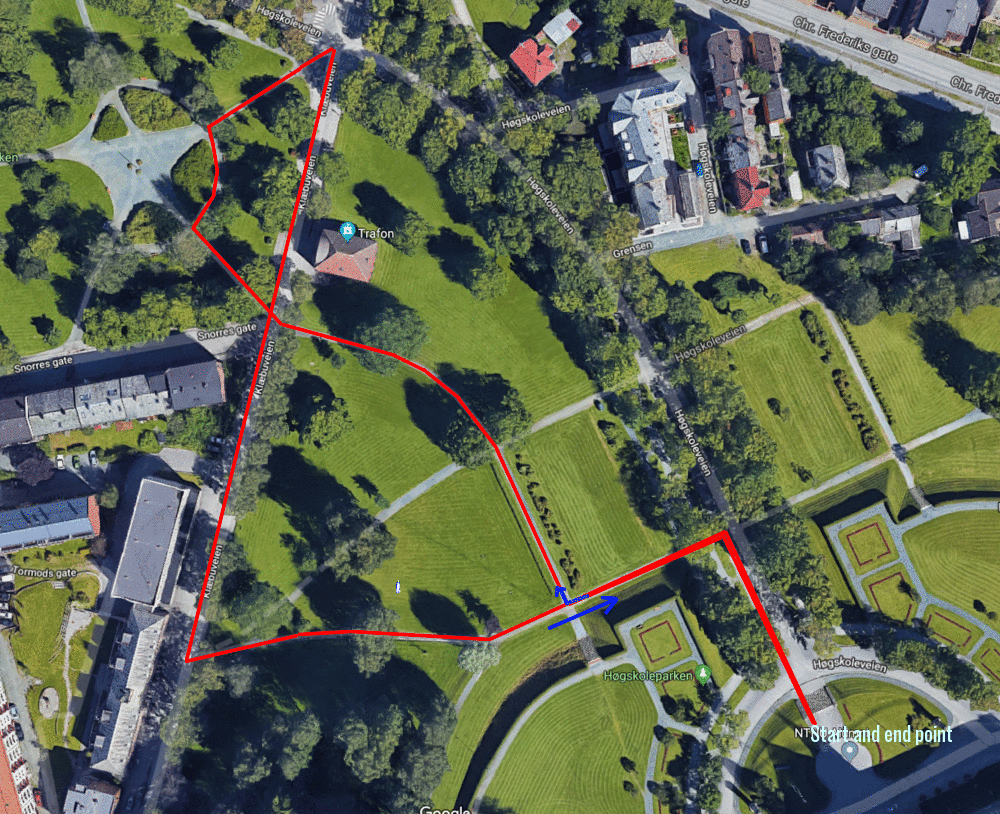
\includegraphics[scale=0.2]{Results/Images/sat-path.png}
        \caption{Satellite image of the test area}
        \label{fig:sat-path}
    \end{figure}
    
%Test location
All of the results presented were gathered from tests performed in the area near the Norwegian university of science and technology. All tests were carried out on foot, with the hardware in hand. Figure \ref{fig:sat-path} shows a satellite image of the area where the test was undertaken, the planned path in red, and the blue arrows indicating the direction walked.\\

A post-processed RTK solution has been used as a reference for position and velocity, where a base station log was acquired online. The base station, positioned approximately 6.5 km away from the testing area, is assumed to be close enough to obtain a reliable solution. RTKLIB does not output velocity and it was orignally planned to use the onboard PixHawk as a reference for velocity estimates, but testing revealed both the position and velocity estimates of the PixHawk to be unusable, and hence no reference for the velocity is provided.\\
%The system was firstly kept stationary, allowing the Kalman filter to converge, and secondly, taken by foot along a path drawn up before testing. The path was laid along a number of small roads to make it easy to follow and thus minimize the difference between it and the actual path taken. 


\section{Stationary tests}
    %Convergence
    %Position cloud
    
    To allow the EKF estimates to converge, the system was kept stationary for 300 seconds before testing was initiated. Results from this process will now be presented.\\
    
    \subsubsection{Position and velocity}
    The stationary position error of the EKF estimate before full convergence and the RTK solution is shown in figure \ref{fig:pos-err-stat}. Note that the RTK solution did not have a fix at this time, and its accuracy can not be trusted completely. Regardless, it does seem to have a better precision than the EKF estimate. After convergence some noise is present, with a precision of approximately 2 meters in the east direction and 5 meters in the the north direction. The EKF is shown to converge after approximately 150 seconds in figure \ref{fig:converge}.\\
    
    \begin{figure}[!htbp]
        \hspace{-1.5cm}
        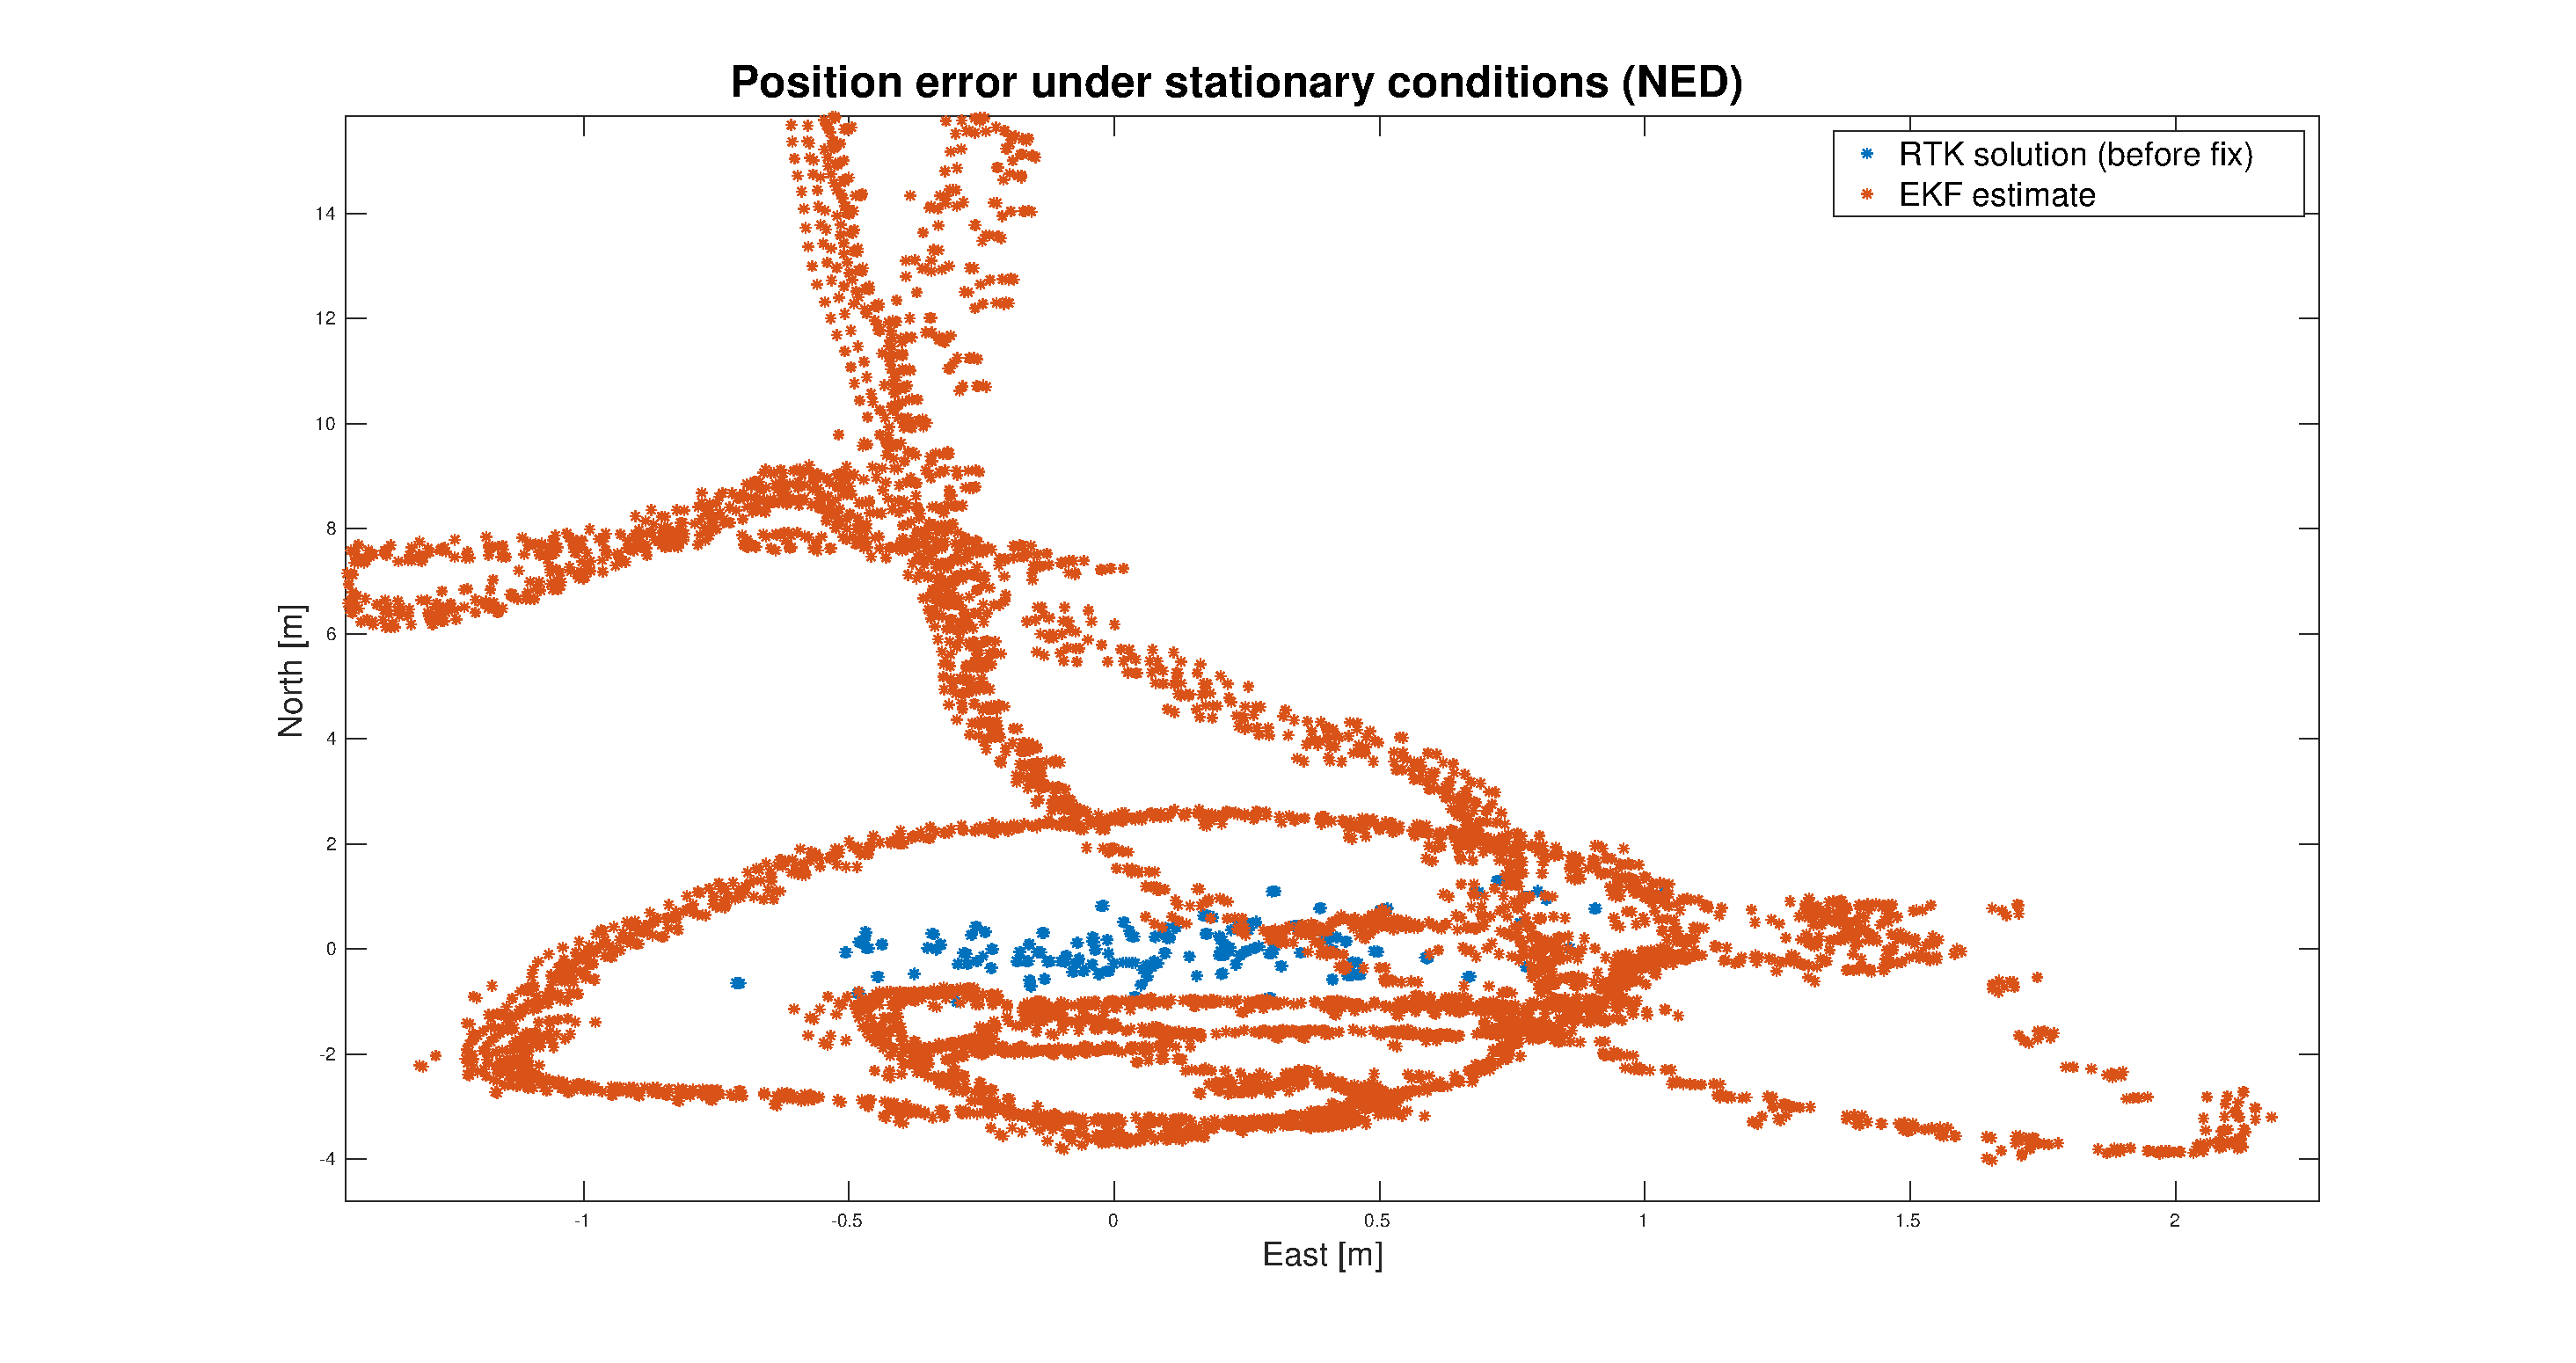
\includegraphics[scale=0.3]{Results/Images/pos-cloud.eps}
        \caption{Cloud plot of the position error under stationary conditions}
        \label{fig:pos-err-stat}
    \end{figure}
    
    \begin{figure}
        \hspace{-1.5cm}
        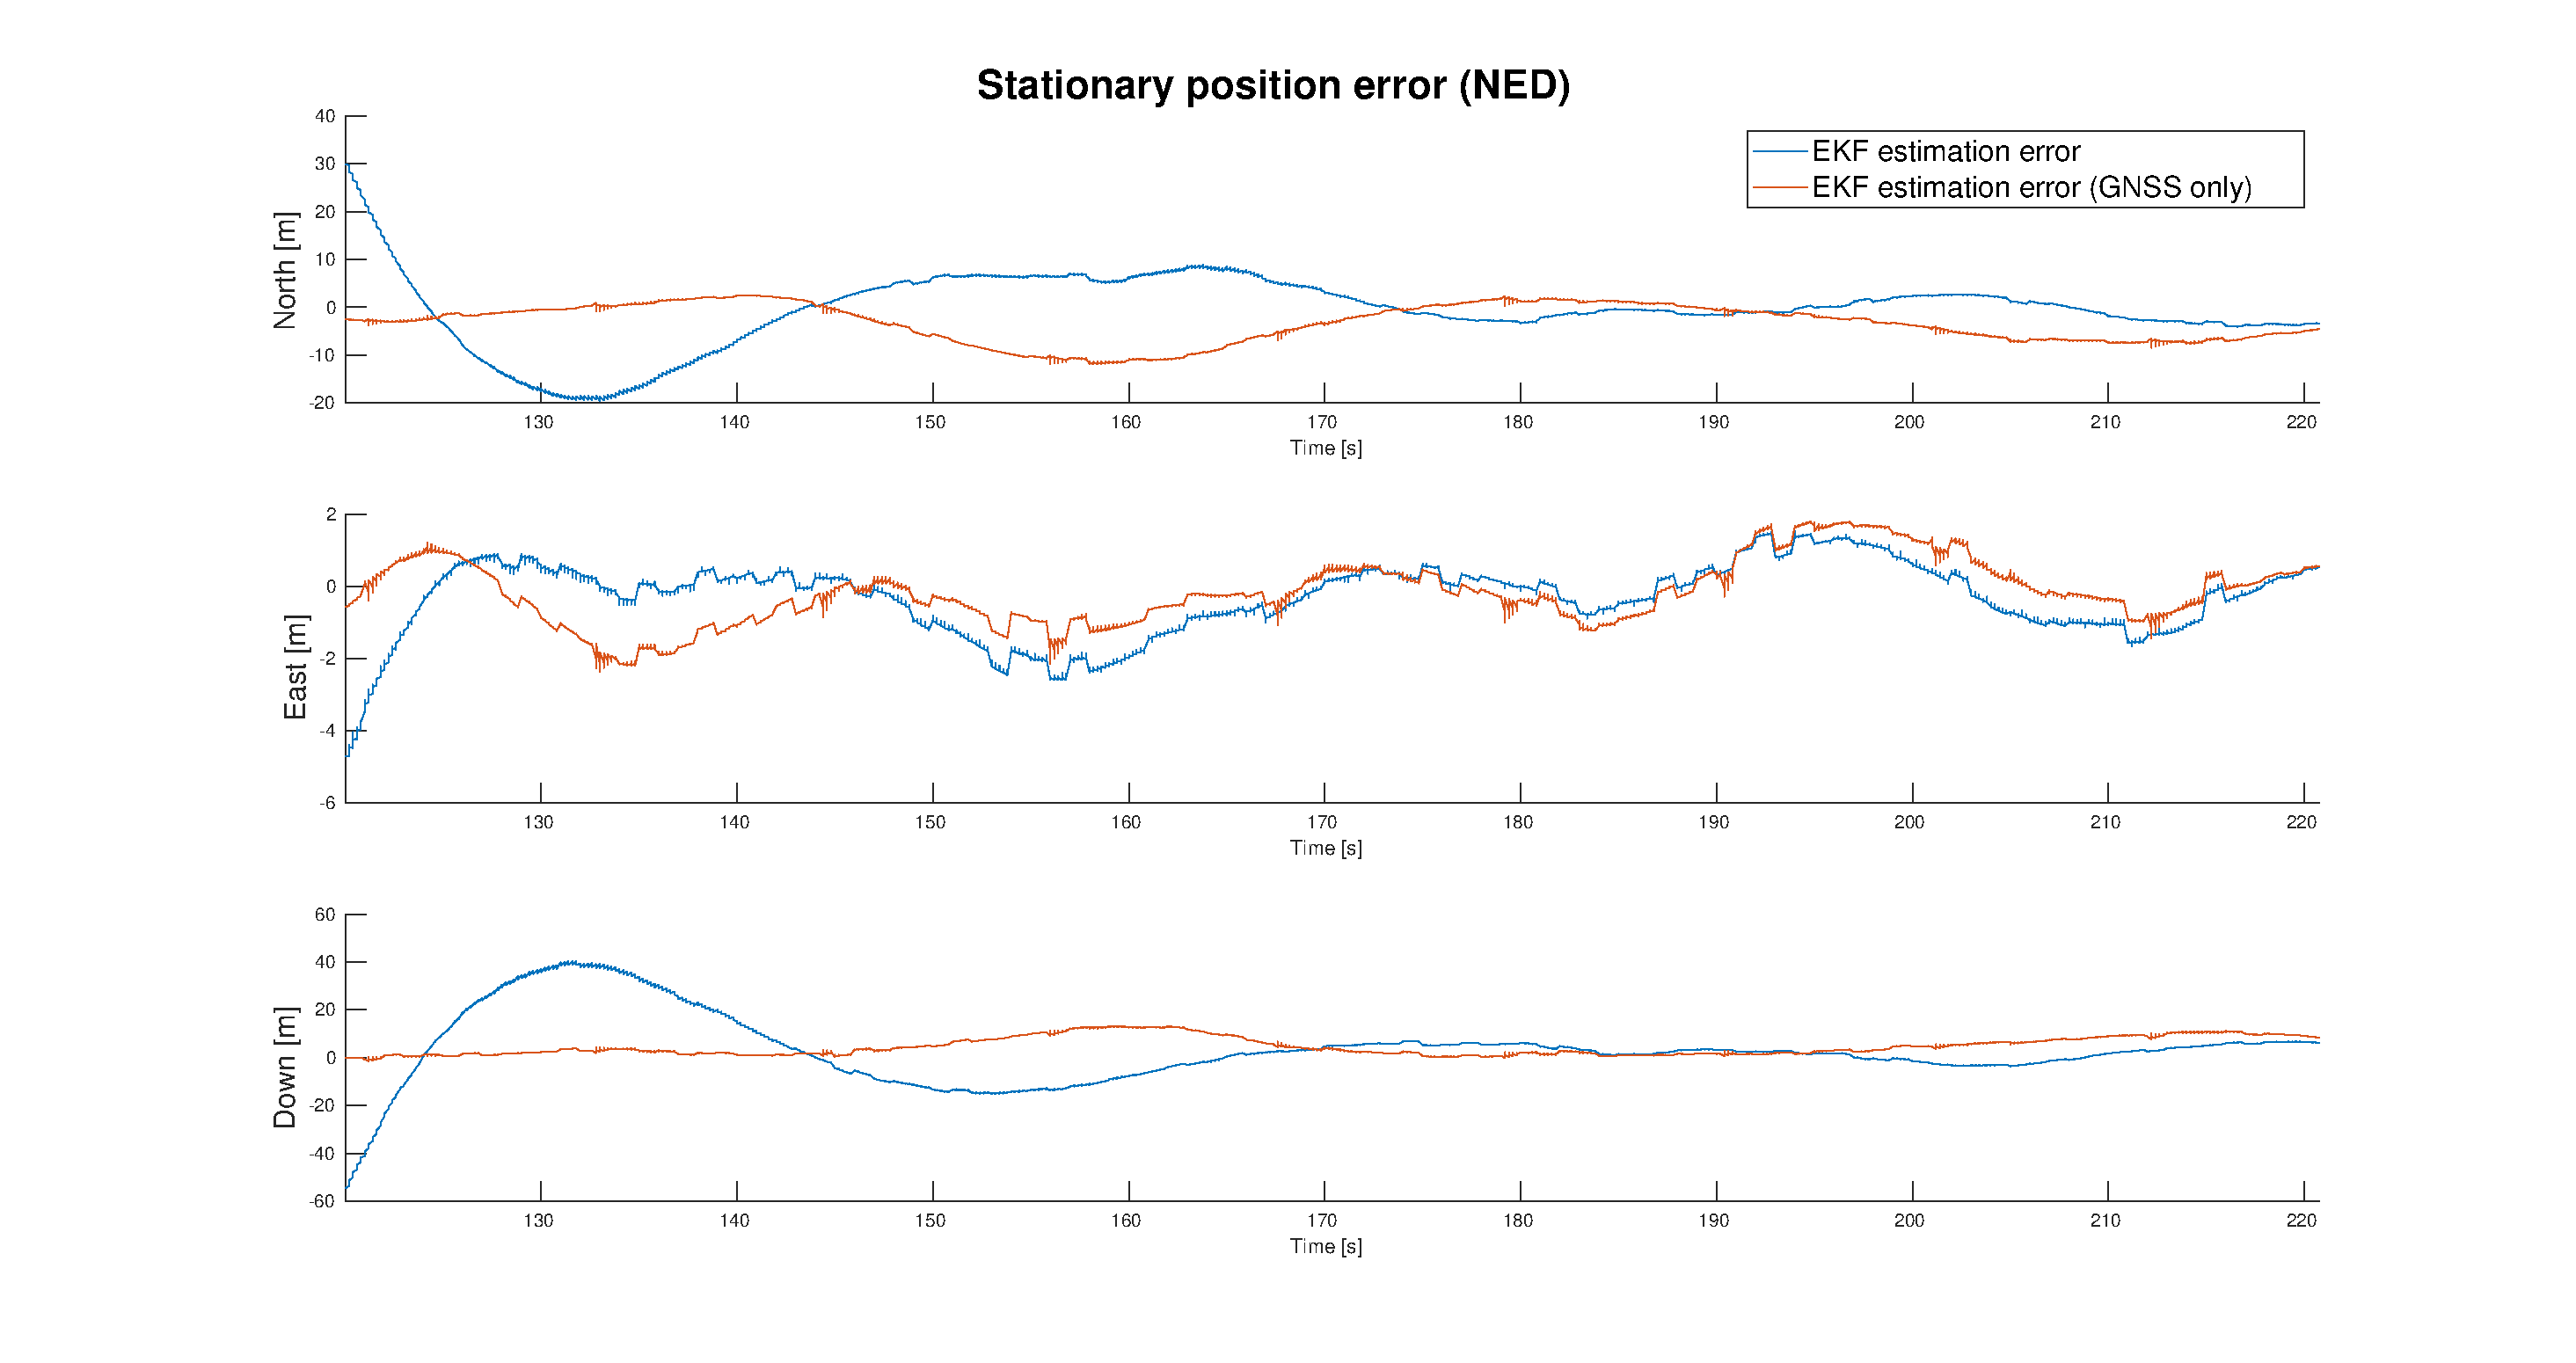
\includegraphics[scale=0.3]{Results/Images/converge.eps}
        \caption{Position error during stationary conditions in three dimensions.}
        \label{fig:converge}
    \end{figure}
    
    The velocity errors of running the EKF with and without acceleration measurements are shown in figure \ref{fig:vel-err-stat}. The solution based solely on GNSS contains some high frequency noise components, and has a root mean square error of $\begin{bmatrix} 0.3701  &  0.1398  &  0.4053\end{bmatrix}$ for north, east and down directions, repectively. Correspondingly, the full system has a root mean square error of $\begin{bmatrix} 1.3830  &  0.1637 &   2.9501\end{bmatrix}$.
    
    \begin{figure}
        \hspace{-1.5cm}
        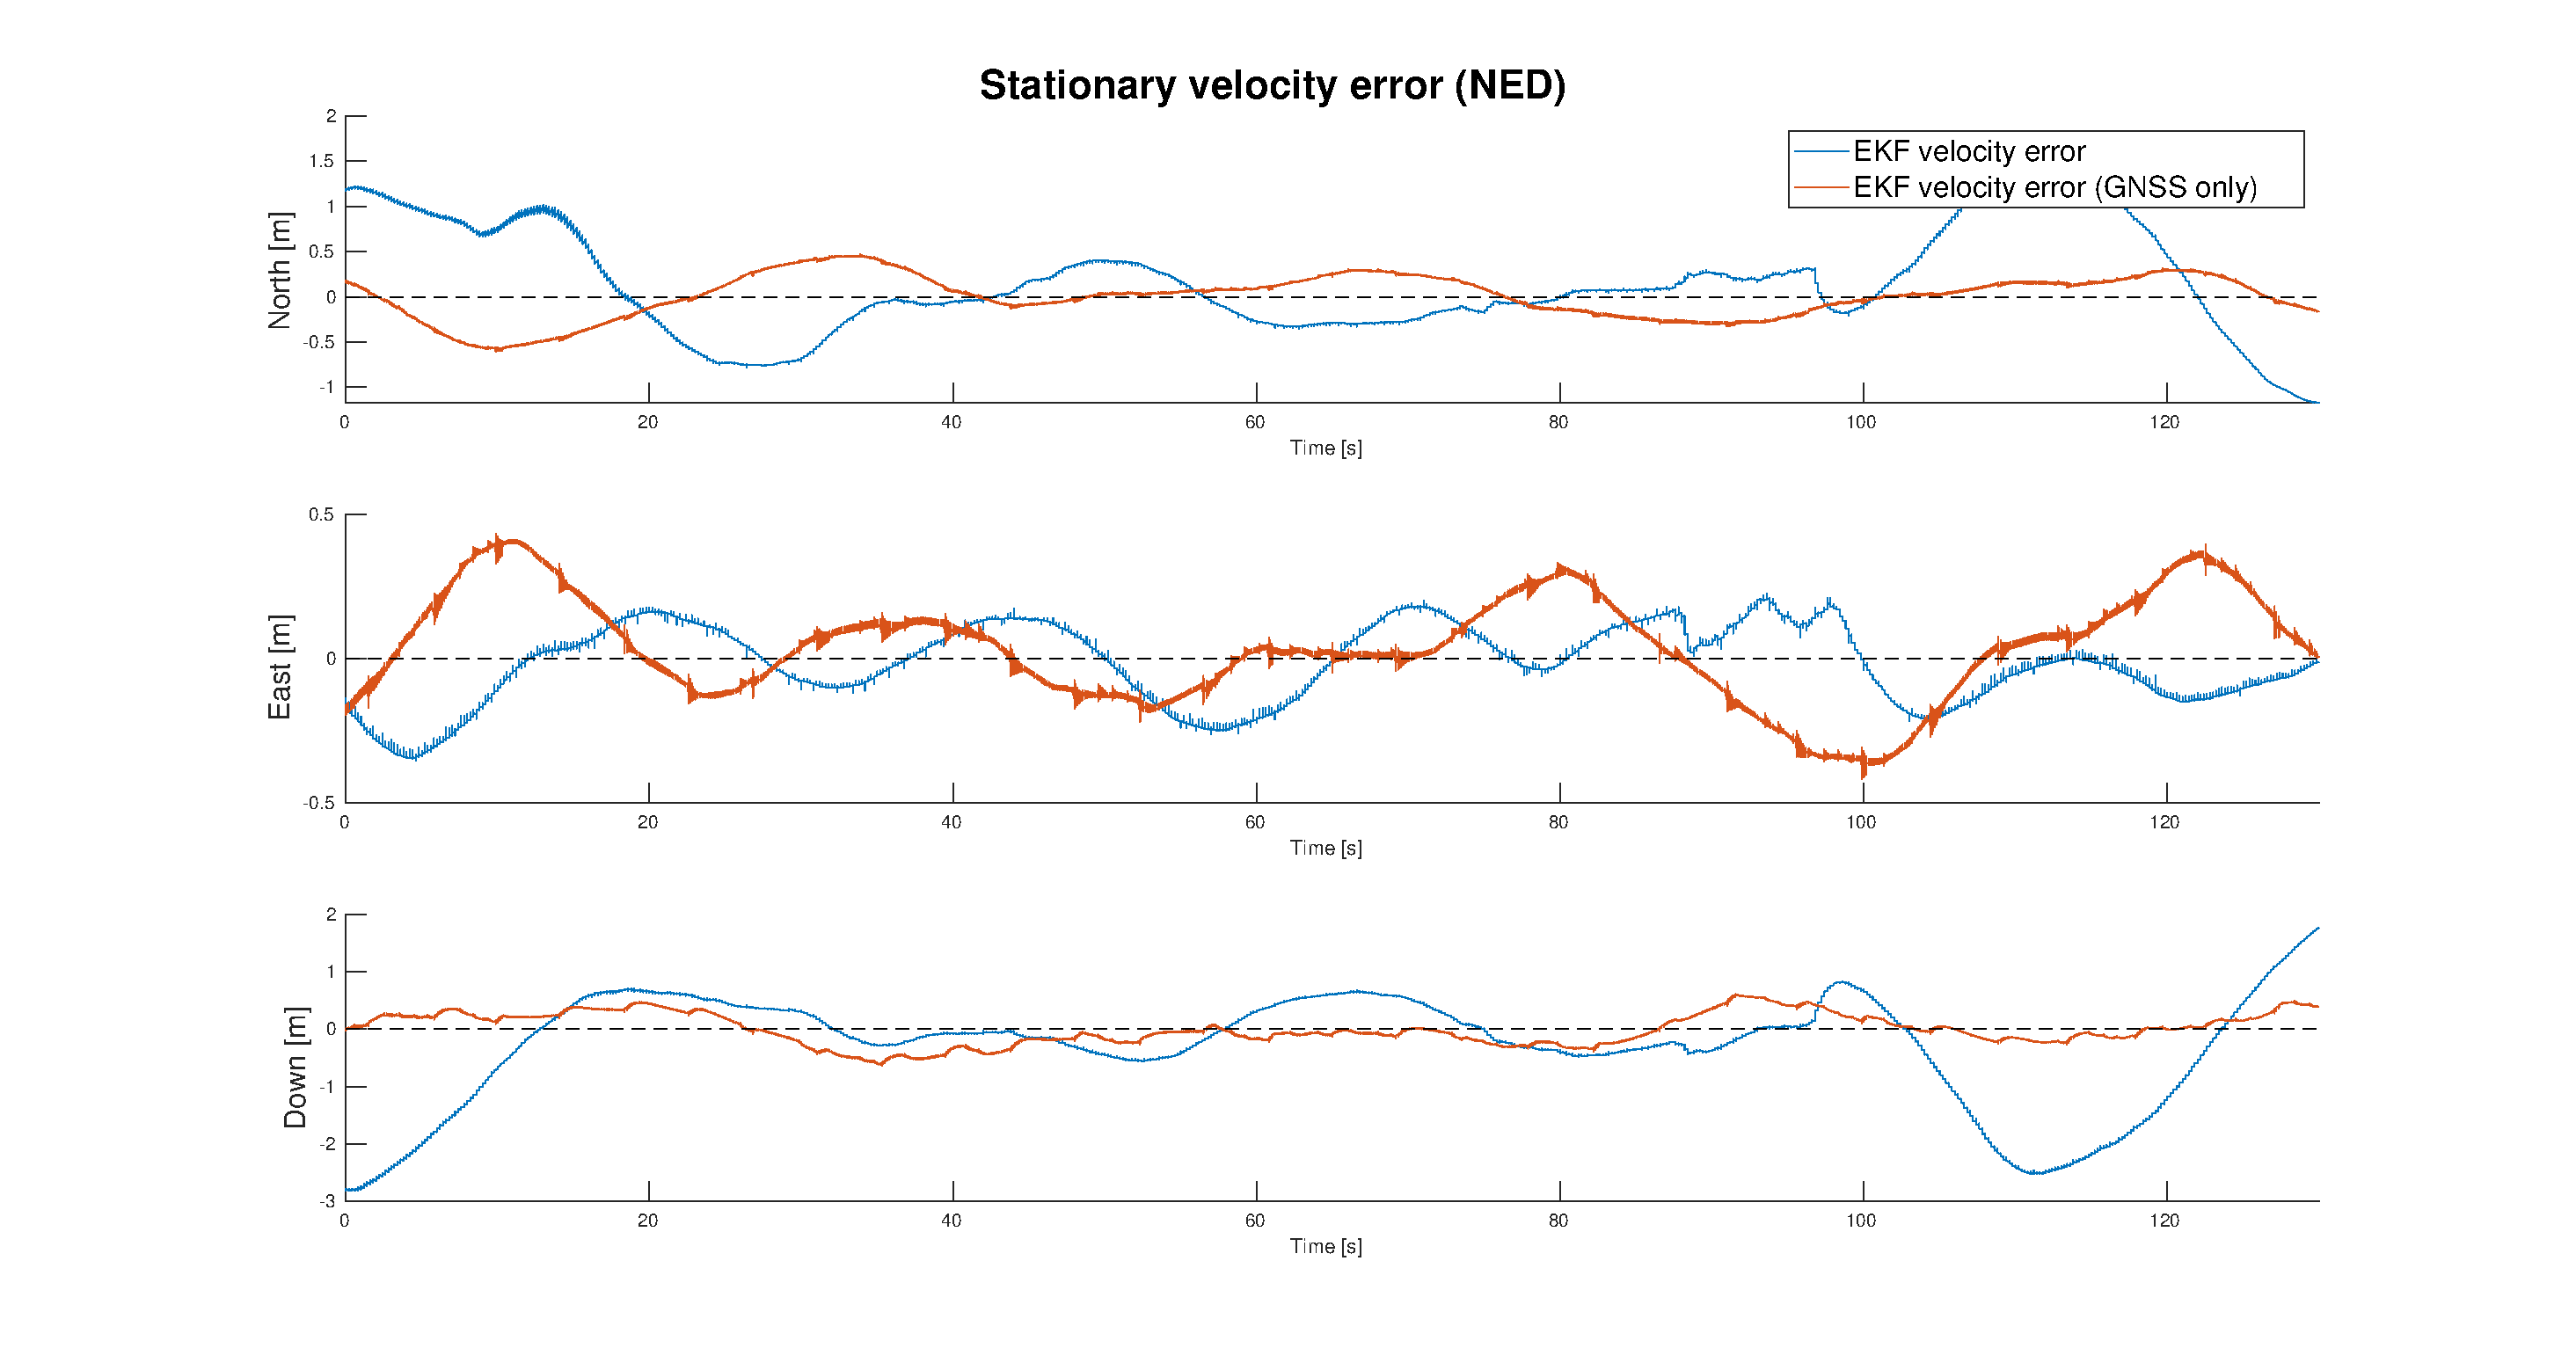
\includegraphics[scale=0.3]{Results/Images/vel-err.eps}
        \caption{Velocity errors of the stationary systems}
        \label{fig:vel-err-stat}
    \end{figure}
    
    \subsubsection{Biases}
    It is important to have a good estimate of the receiver clock bias to get any meaningful results from the GNSS. This estimate is shown in figure \ref{fig:bias} and, as expected, is shown to have a constant slope after convergence. The estimated rate of the receiver clock bias is shown in figure \ref{fig:bias-rate-stat} with and without acceleration measurements. While the solution based on GNSS only contains low frequency spikes, the tightly coupled estimate contains some higher frequency noise components.\\
    
    \begin{figure}
        \hspace{-1.5cm}
        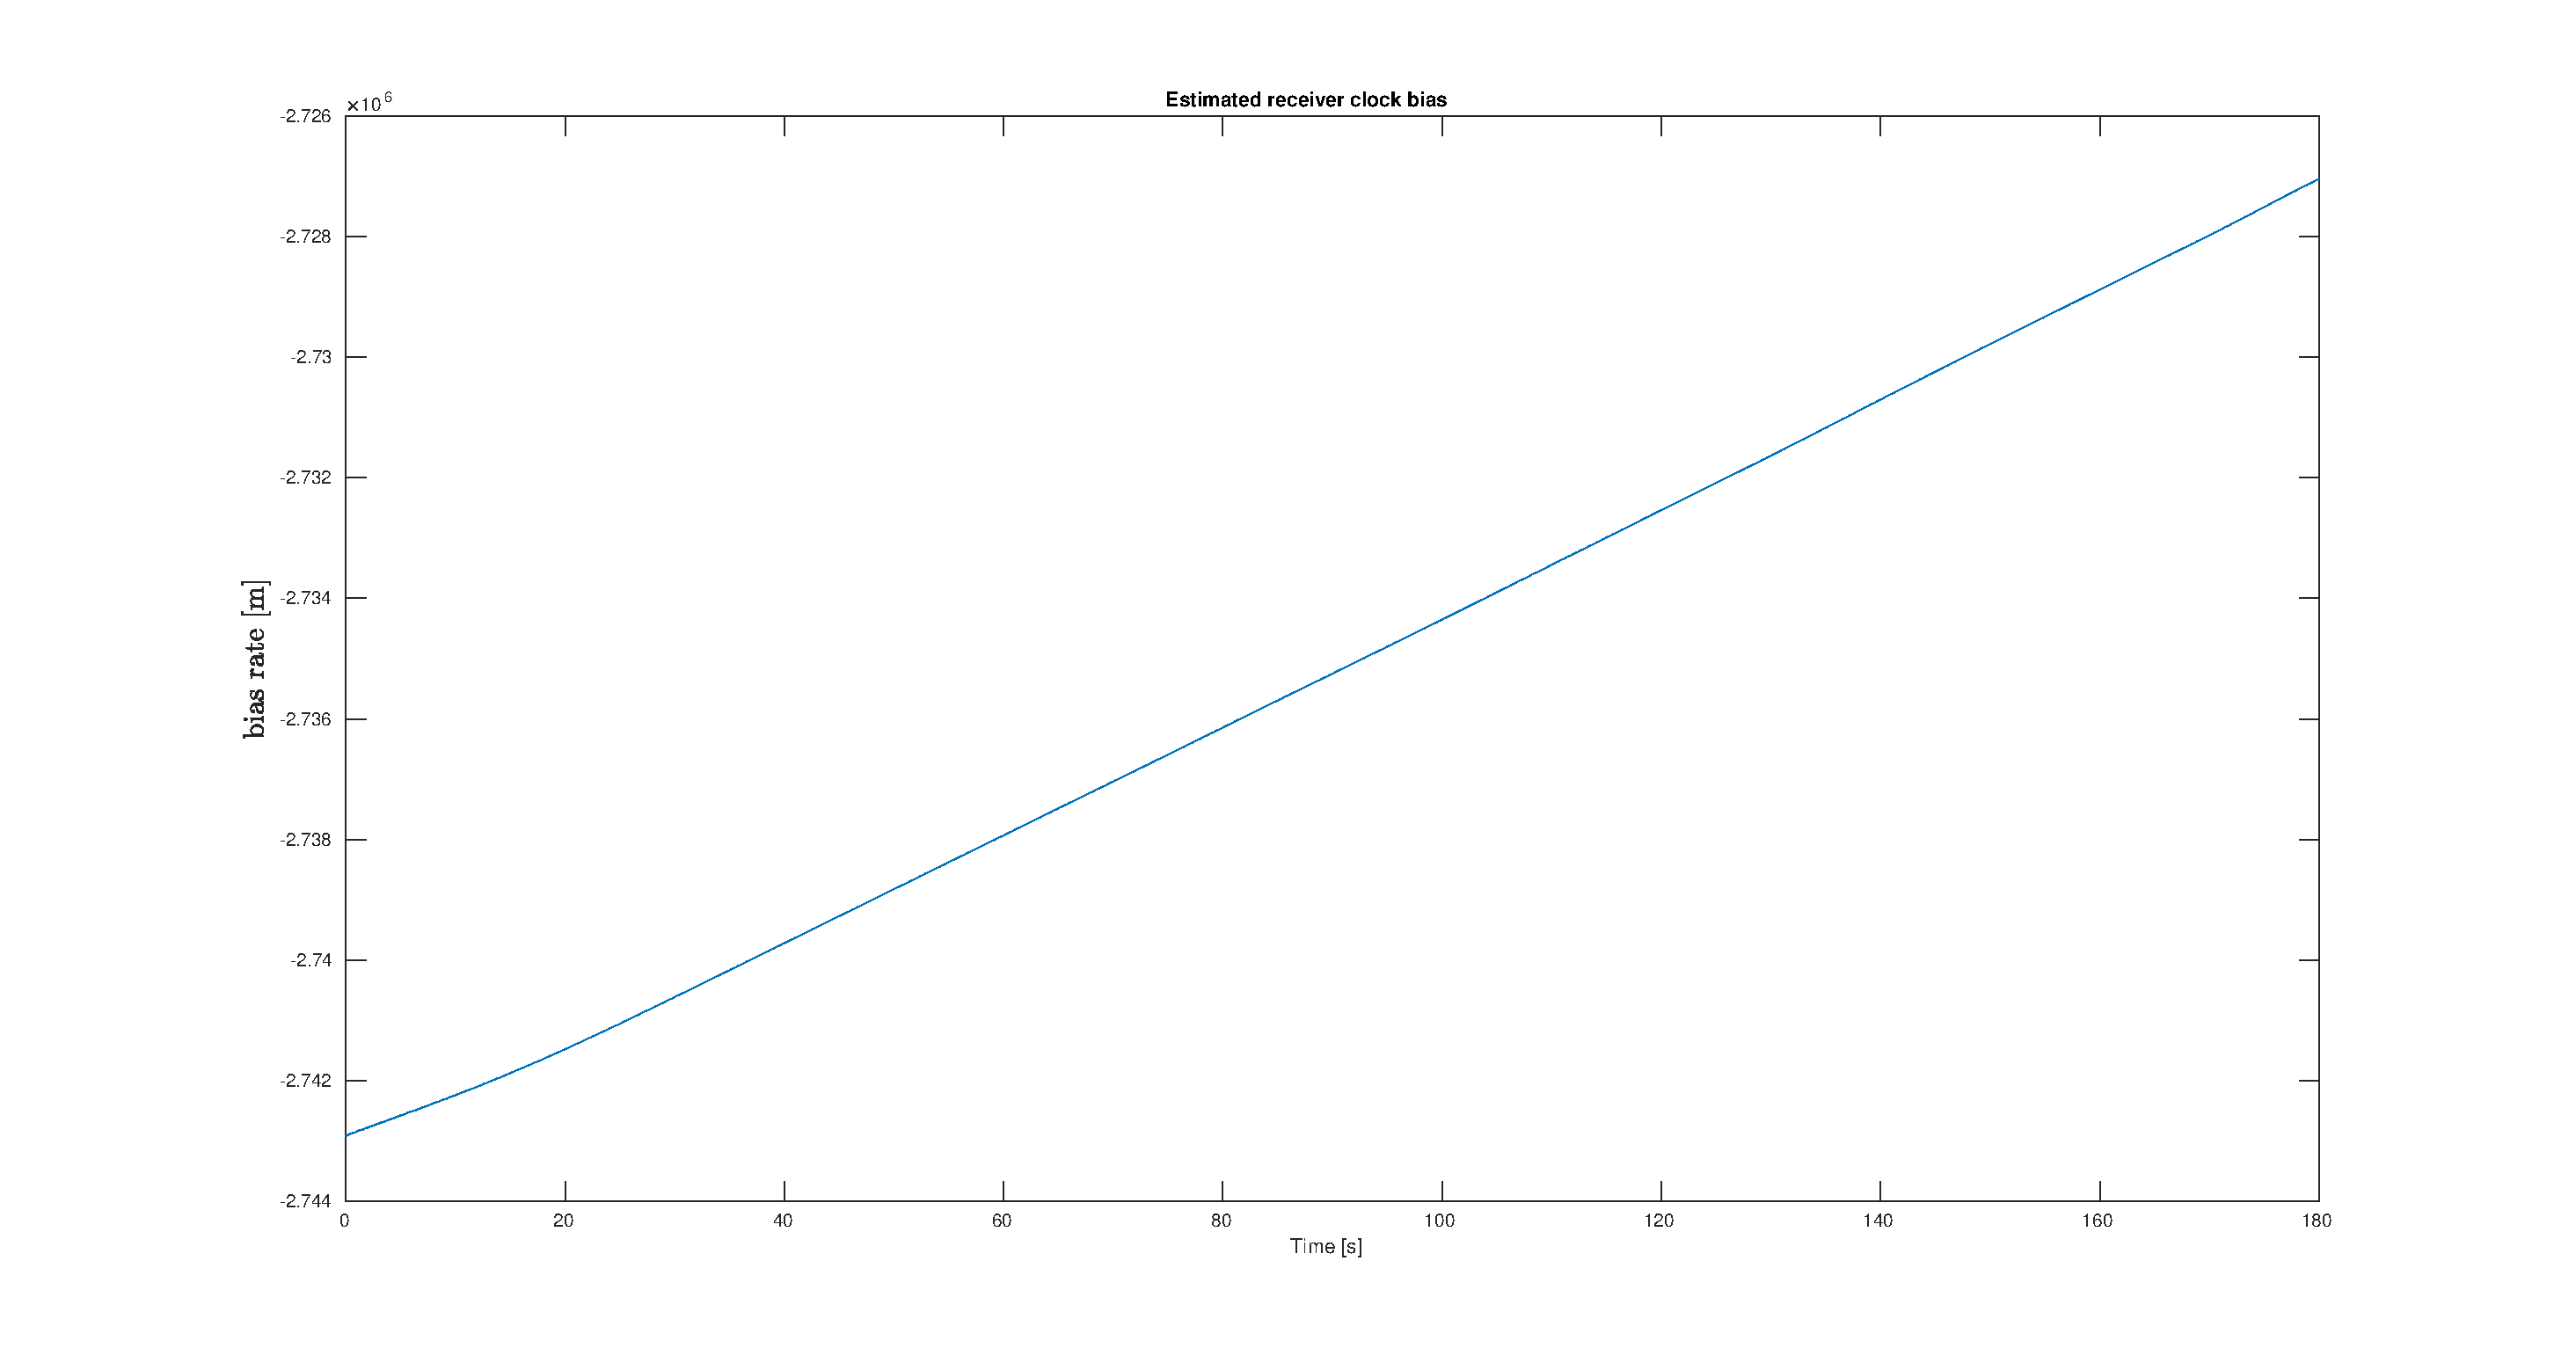
\includegraphics[scale=0.3]{Results/Images/bias.eps}
        \caption{Receiver clock bias}
        \label{fig:bias}
    \end{figure}
    
    \begin{figure}
        \hspace{-1.5cm}
        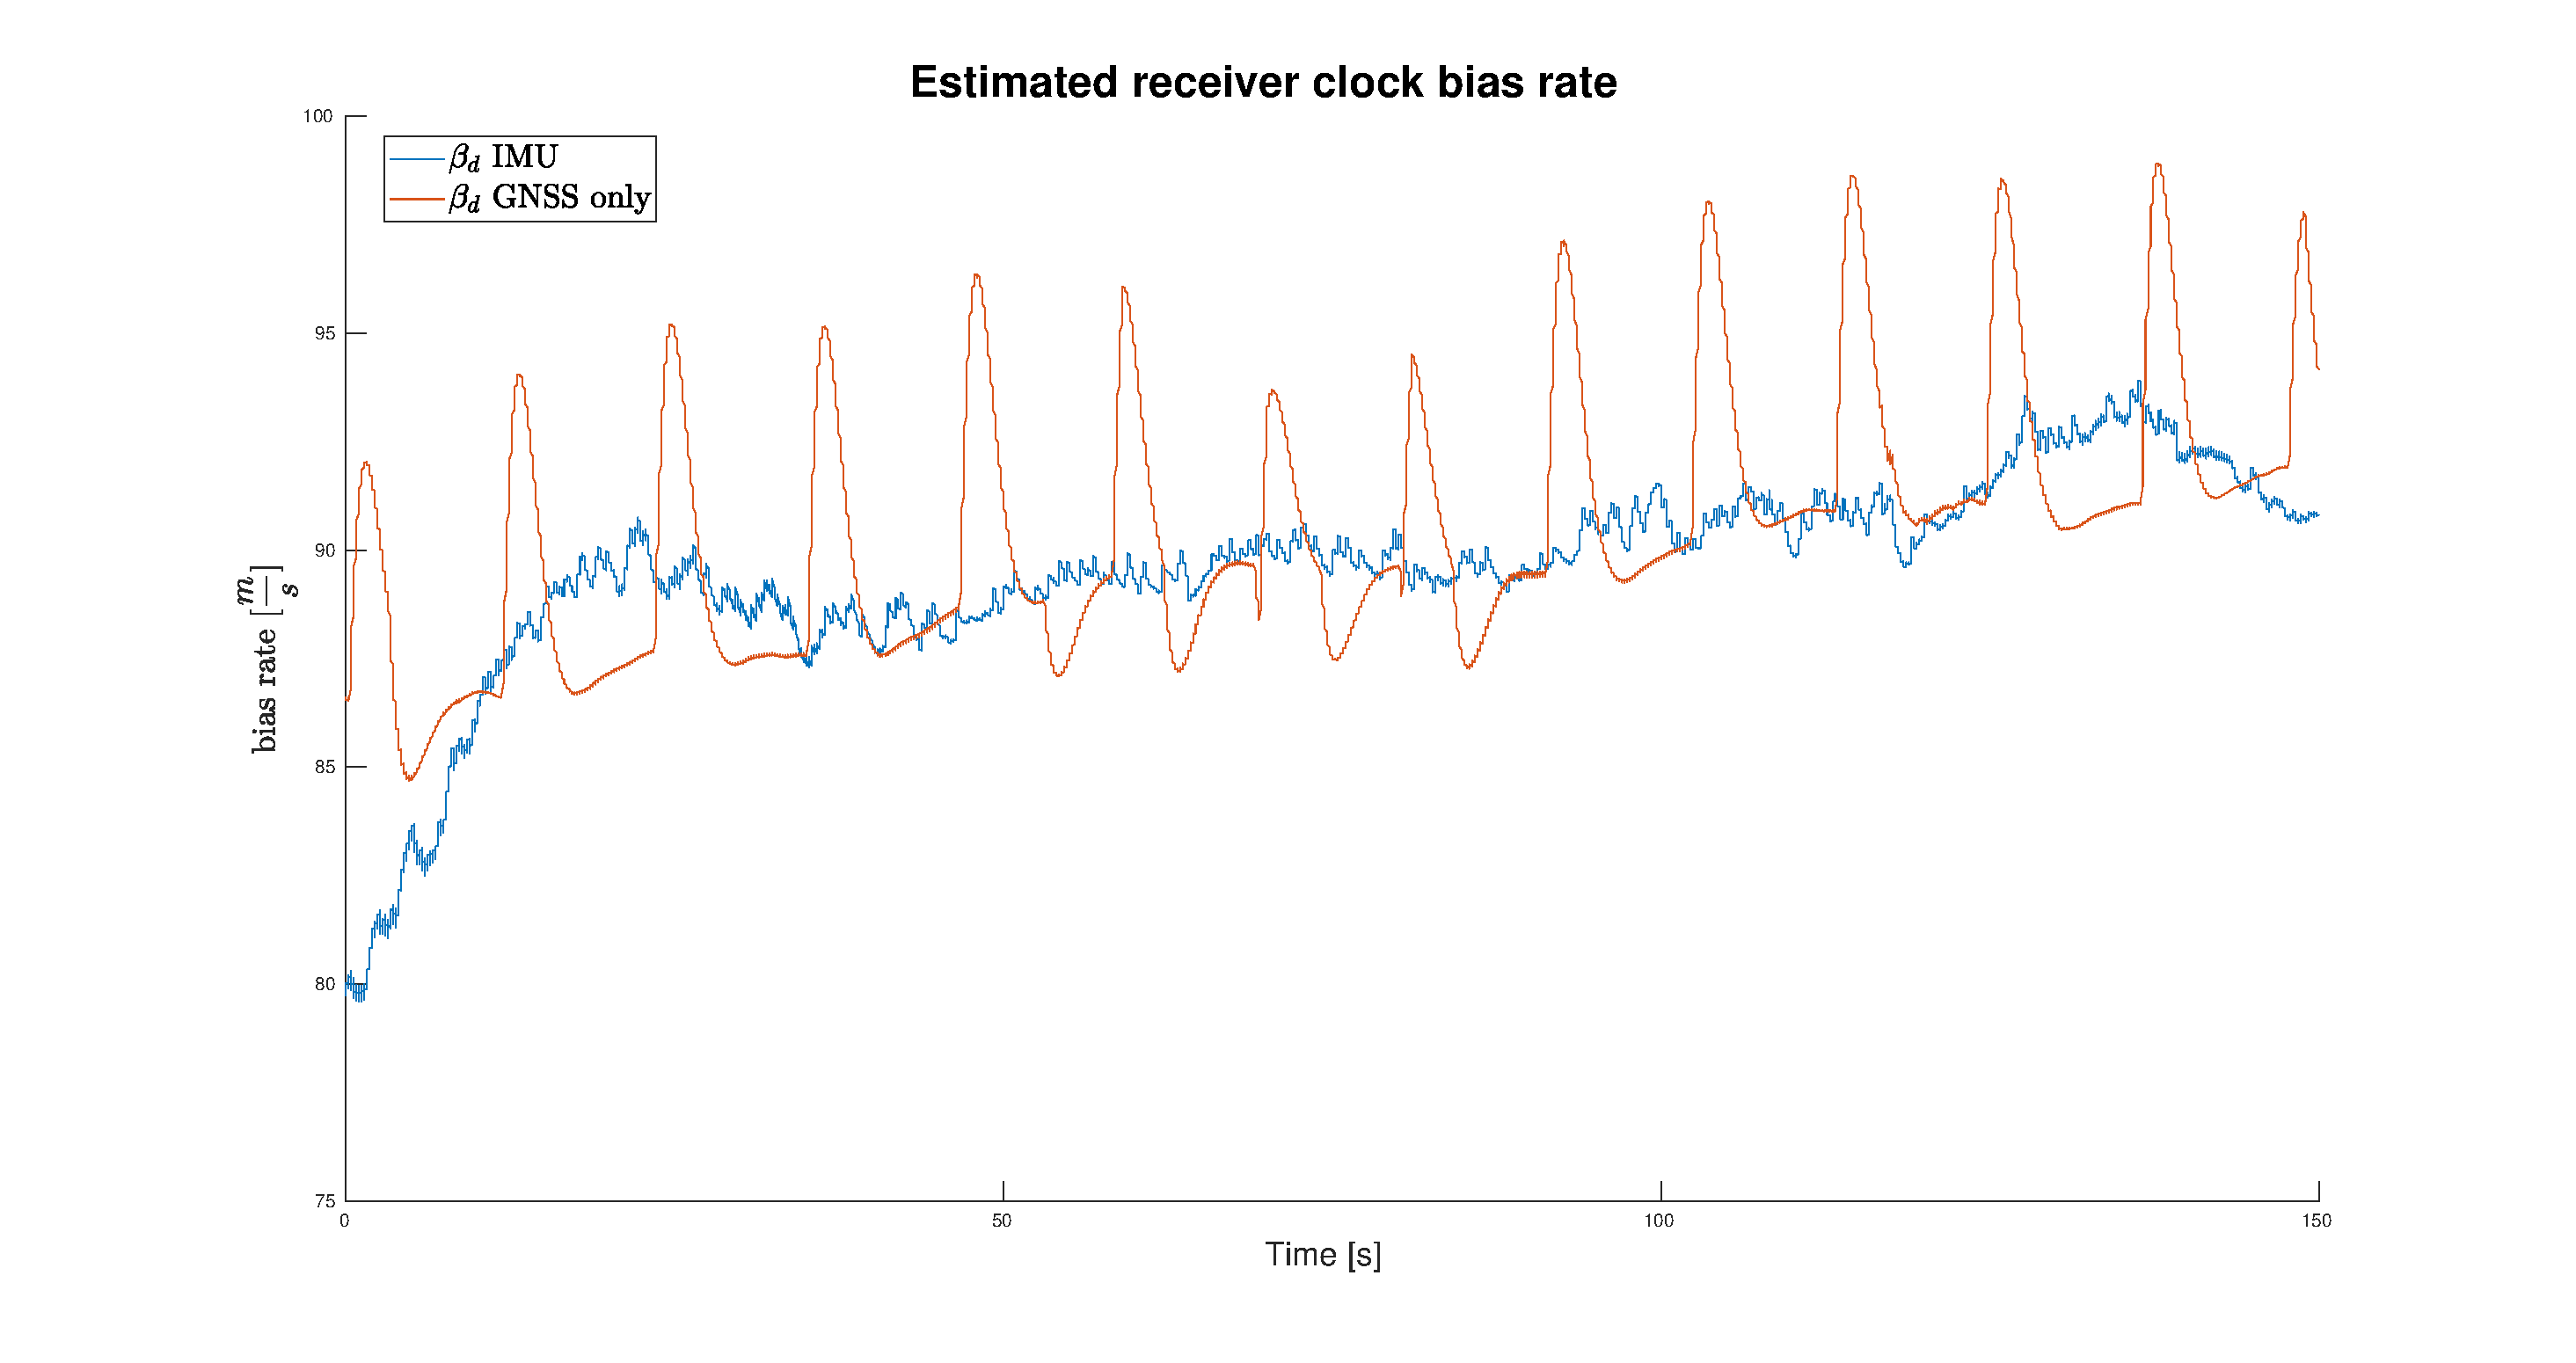
\includegraphics[scale=0.3]{Results/Images/bias_rate-stat.eps}
        \caption{Receiver clock bias rate of the tightly coupled system when stationary.}
        \label{fig:bias-rate-stat}
    \end{figure}
    
    It was found that the PixHawk IMU measurements contained fairly significant biases, important to estimate to achieve reliable results. This estimate is plotted together with acceleration measurements in figure \ref{fig:bias-acc}. Note that the measurements are corrected for gravity. It is seen from the plot that the EKF makes a fair approximation of the bias.\\
    
    \begin{figure}[!htbp]
        \hspace{-1.5cm}
        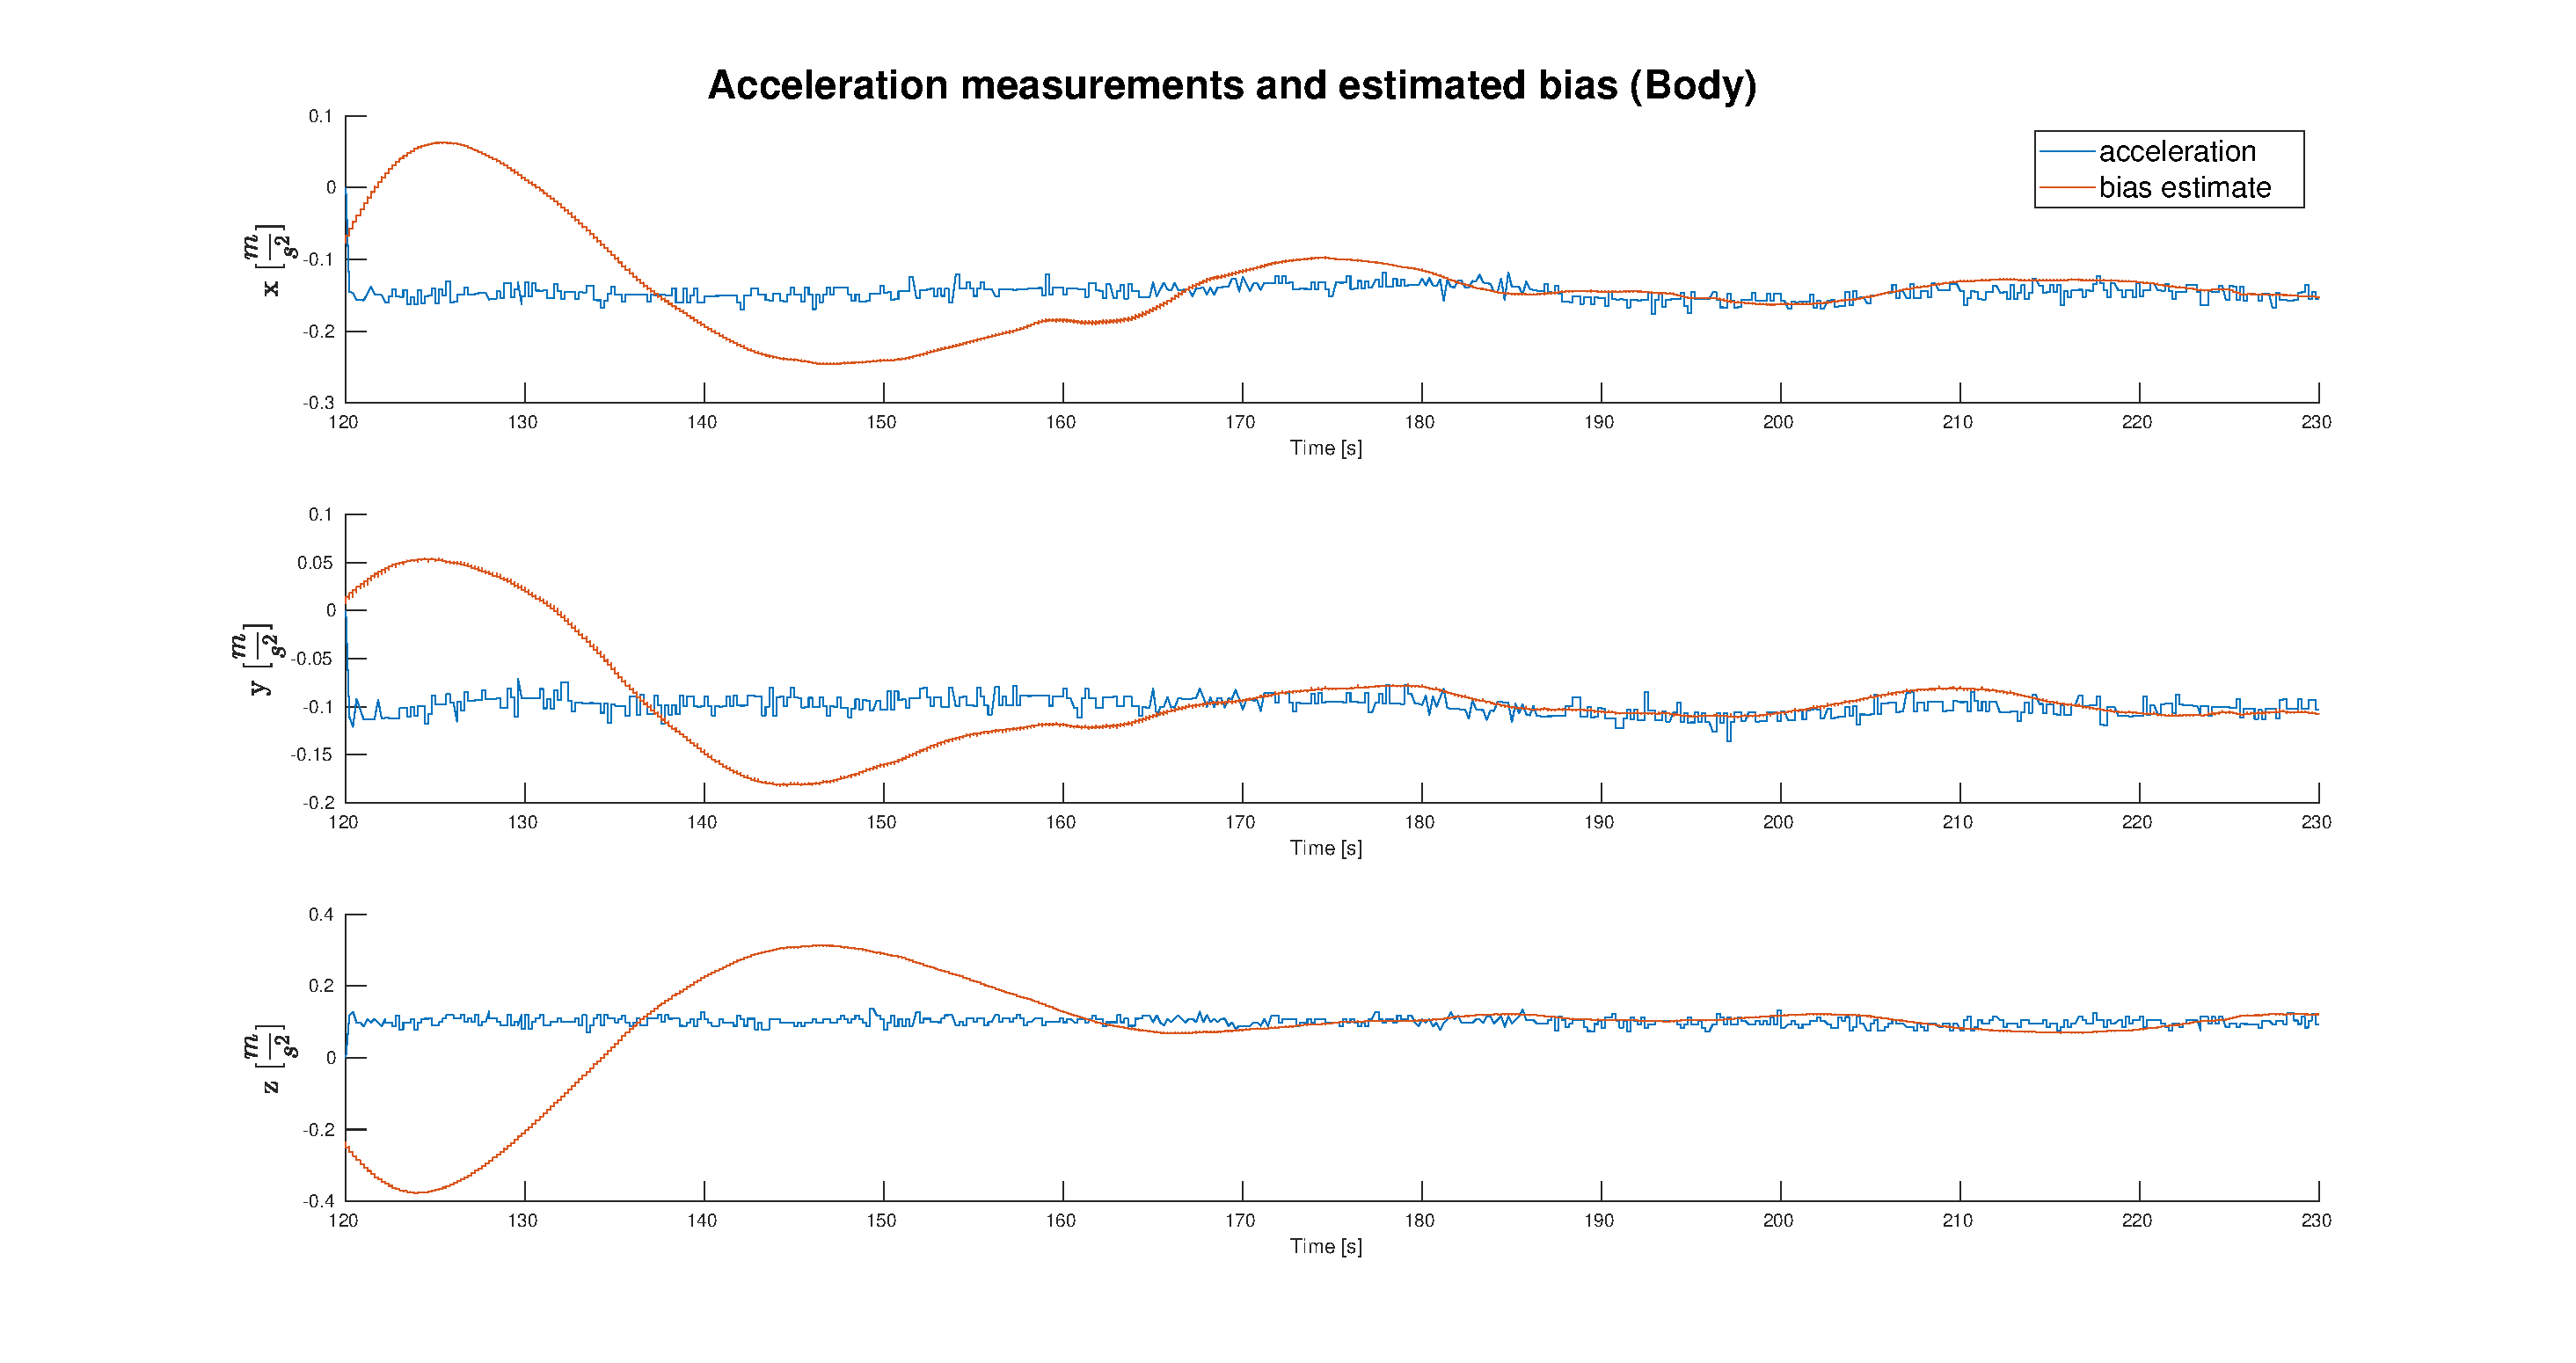
\includegraphics[scale=0.3]{Results/Images/bias-acc.eps}
        \caption{Estimated accelerometer bias with uncorrected acceleration measurements}
        \label{fig:bias-acc}
    \end{figure}
    
\section{Dynamic tests}
    This section covers the part of testing where the system was in motion. To further look into the the benefits of applying acceleration measurements to the EKF, the planned test was performed twice under different conditions. First, the full EKF was run with acceleration and GPS measurements at a frequency of 5 Hz, with results presented in section \label{sec:res:tightly-coupled}. Second, the GNSS receiver was configured to output both GPS and GLONASS measurements at 10 Hz, while the acceleration measurements were discarded, leading to state estimates based on GNSS only. These results are presented in section \label{sec:res:multi-gnss}.\\
    
    %The system was tested without any IMU-measurements. The GNSS receiver was configured to output GPS and GLONASS pseudo-range and doppler measurements at a 10 Hz frequency. The estimated latitude and longitude are show in figure \ref{fig:test-gnss}.\\
    

    %GNSS only compared with reference path
    %velocity quiver plots in map
    %The full system used GPS measurements only, at a frequency of 5 Hz. This was done to lighten computational load, as the IMC-logging module was prone to crashing during the test, rendering the logs useless. Figure \ref{fig:full-pos-sub} plots the position estimates of the EKF and the PixHawk, and compares these to the RTK reference. Surprisingly, the PixHawk estimates, while smooth, seem to be significantly worse than those of the EKF. 
    \subsection{The tightly coupled system}
    \label{sec:res:tightly-coupled}
    Figure \ref{fig:test-gnss-vel} shows the latitude and longitude estimates with velocity vectors averaged over approximately a second each. The vectors in the lower left corner have a smaller magnitude as this part of the path goes uphill. Assuming course and heading to be equal, the velocity vectors would ideally go tangential to the reference, but as can be seen, this is not always the case.\\
     
    %\begin{figure}[!htbp]
    %    \hspace{-1.5cm}
    %    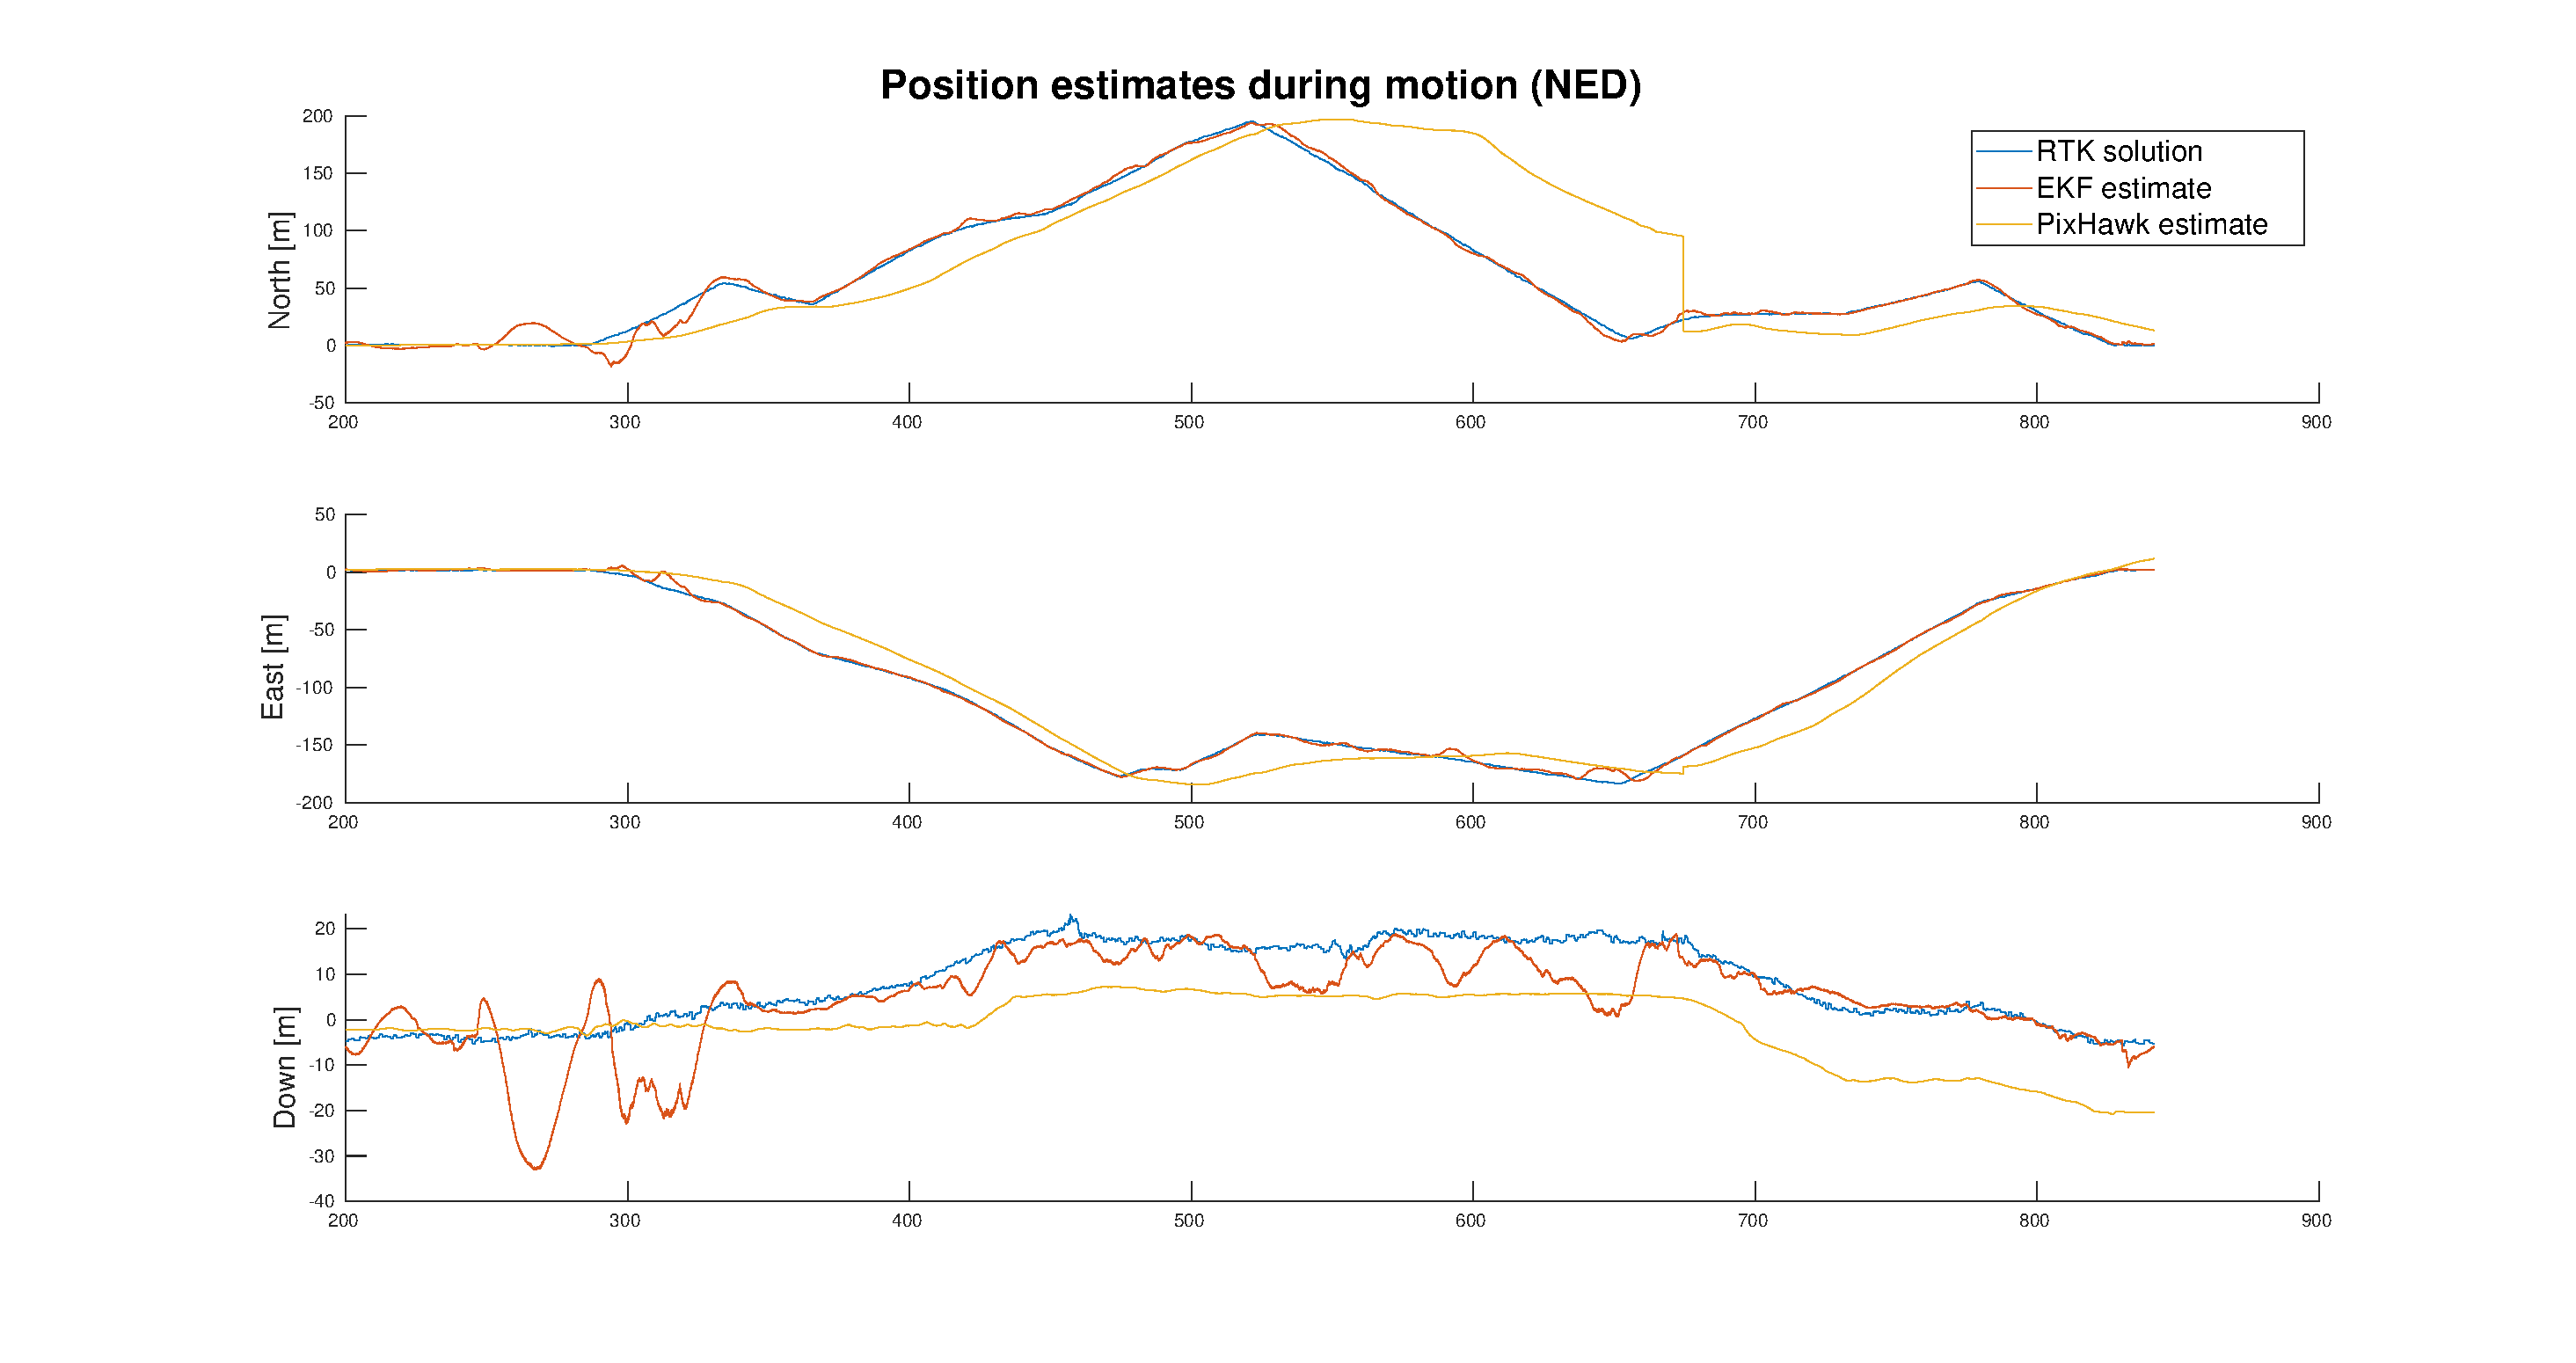
\includegraphics[scale=0.3]{Results/Images/position-sub.eps}}
    %    \caption{Seperate position estimates in NED}
    %    \label{fig:full-pos-sub}
    %\end{figure}
    
    \begin{figure}[!htbp]
        %\centering
        \hspace{-1.5cm}
        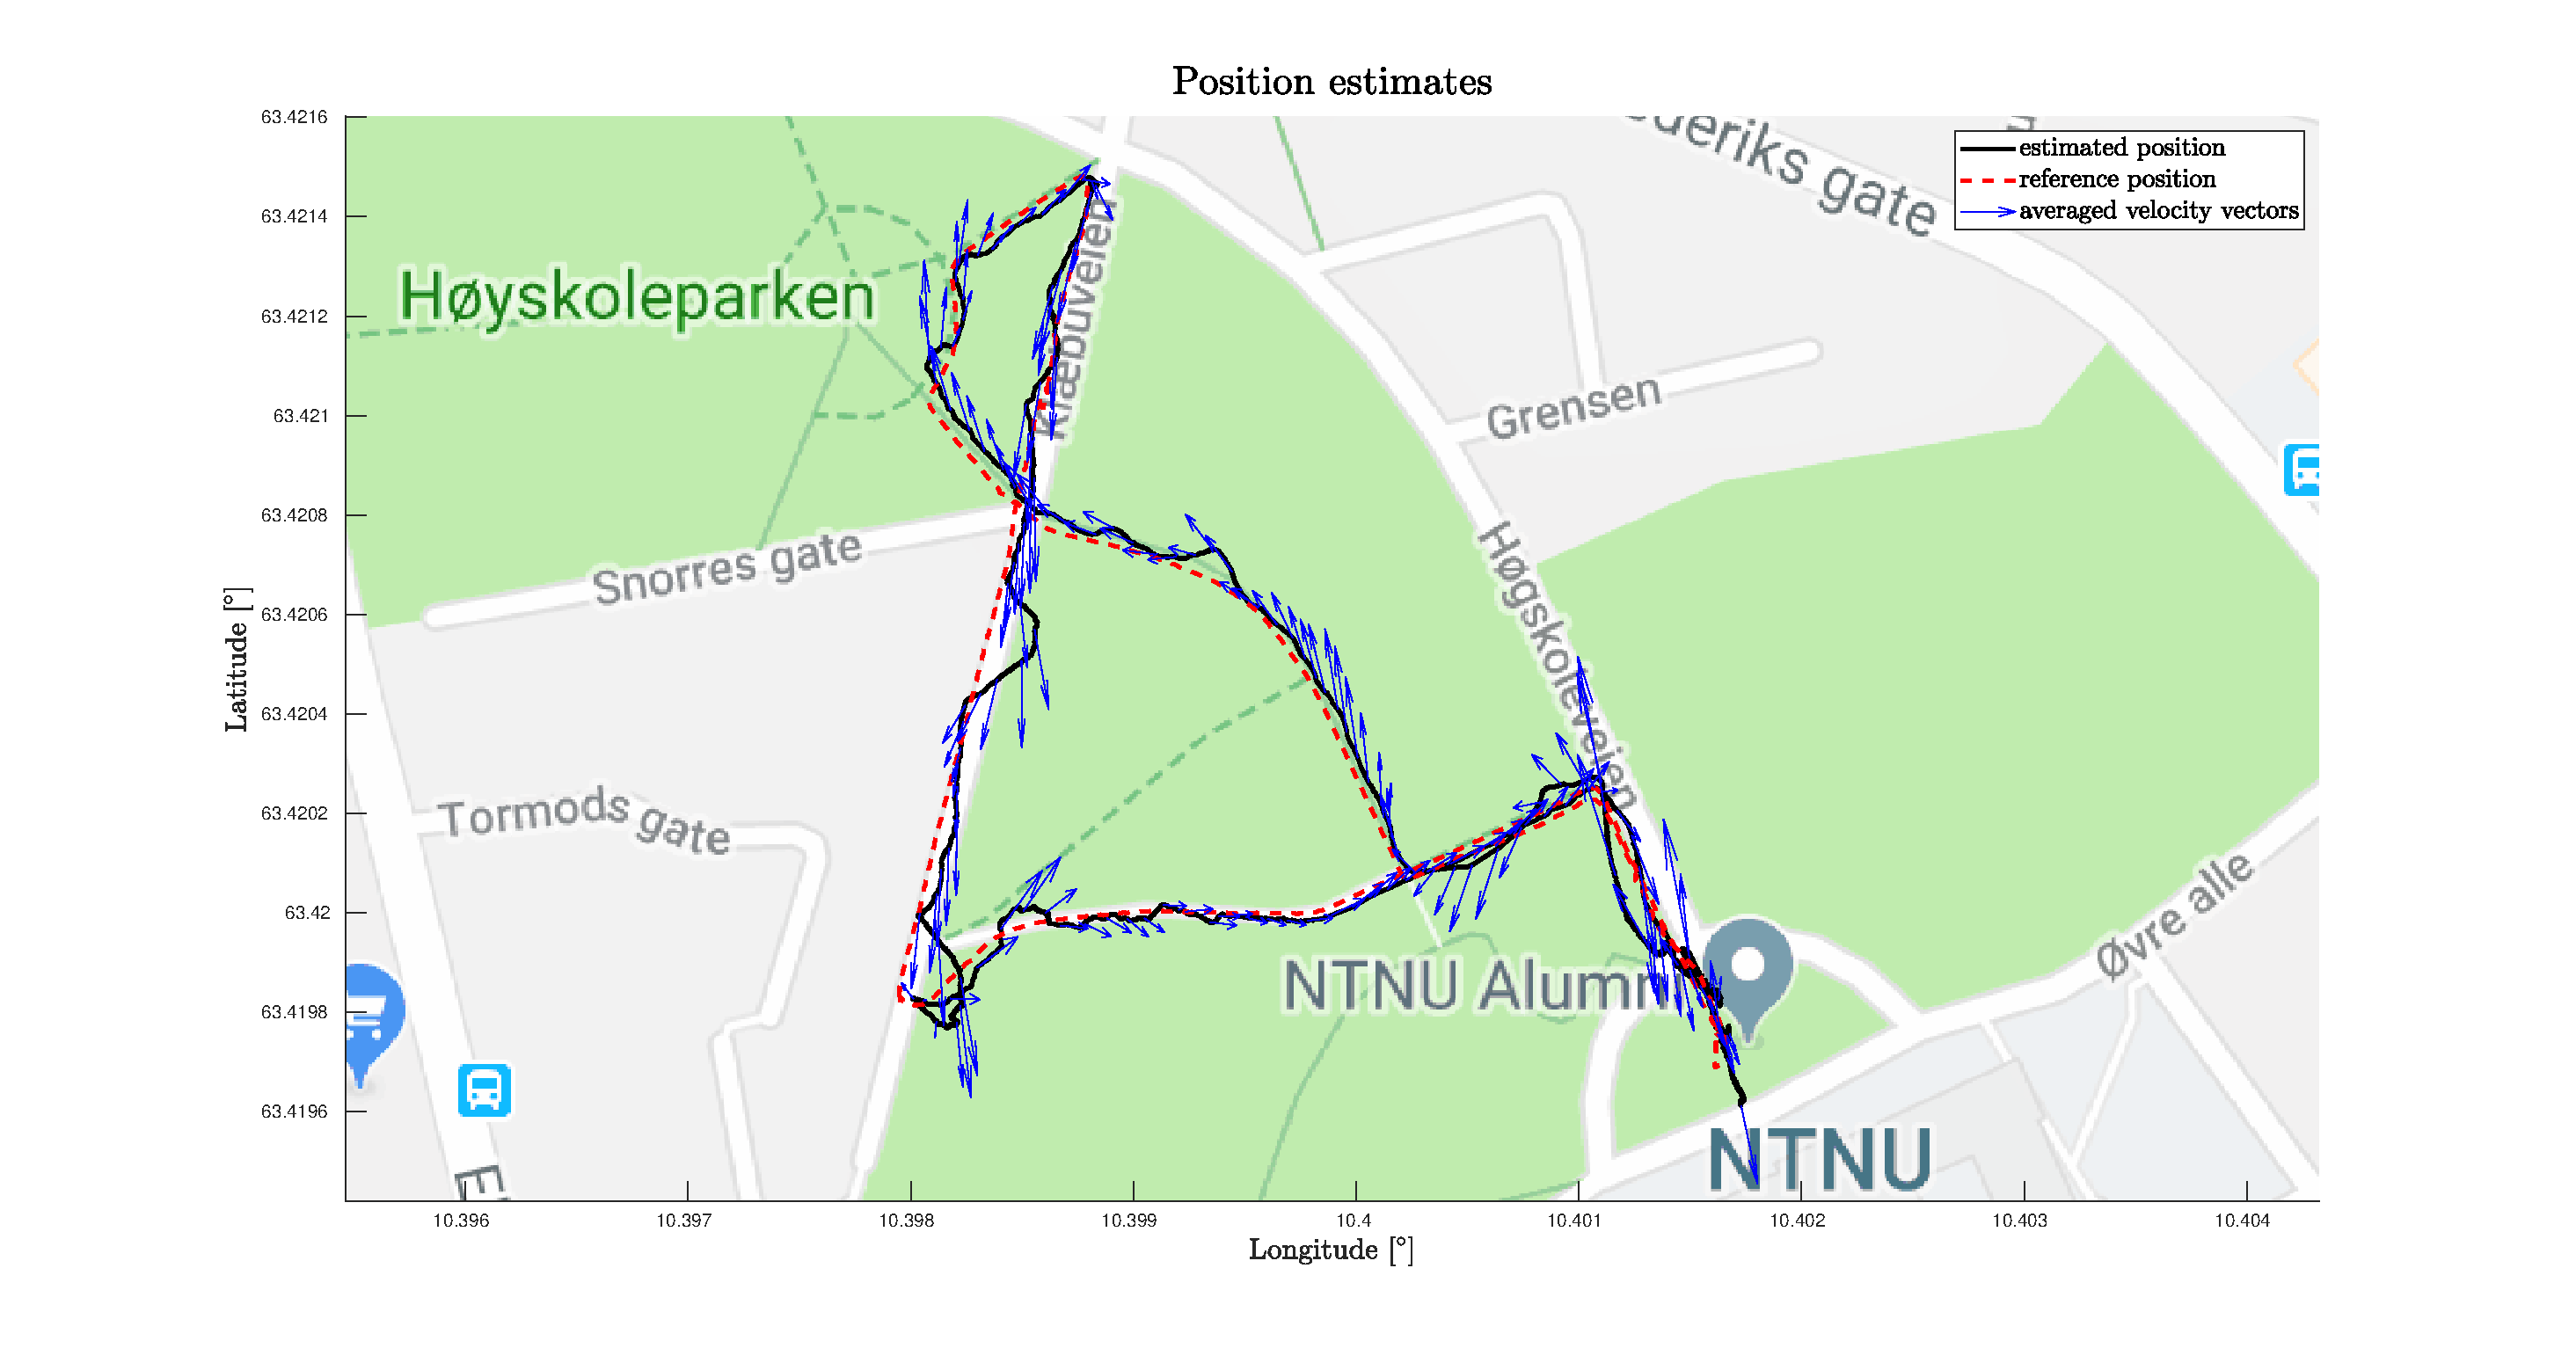
\includegraphics[scale=0.3]{Results/Images/position-with-vel.eps}
        \caption{Position estimates with averaged velocity vectors.}
        \label{fig:test-gnss-vel}
    \end{figure}
    
    The distributions of the position error of both setups are represented as histograms in figures \ref{fig:error-hist} and \ref{fig:error-hist-gnss}. The tightly coupled solution was found to have a root mean square error (RMSE) of $\begin{bmatrix} 5.1192 & 2.5267 & 7.1108\end{bmatrix}$ in the north, east and down direction, respectively, while the purely GNSS based solution had a lower RMSE of $\begin{bmatrix}2.4492 & 1.3123 & 6.3648 \end{bmatrix}$. However, the former is seen to roughly retain a normal distribution, as opposed to the GNSS based estimation errors. At this point, it is also interesting to note how the noise of the receiver clock bias estimate increases significantly when the acceleration measurements are discarded, as shown in figure \ref{fig:bias-rate}.\\
    
    \begin{figure}[!htbp]
        \hspace{-1.5cm}
        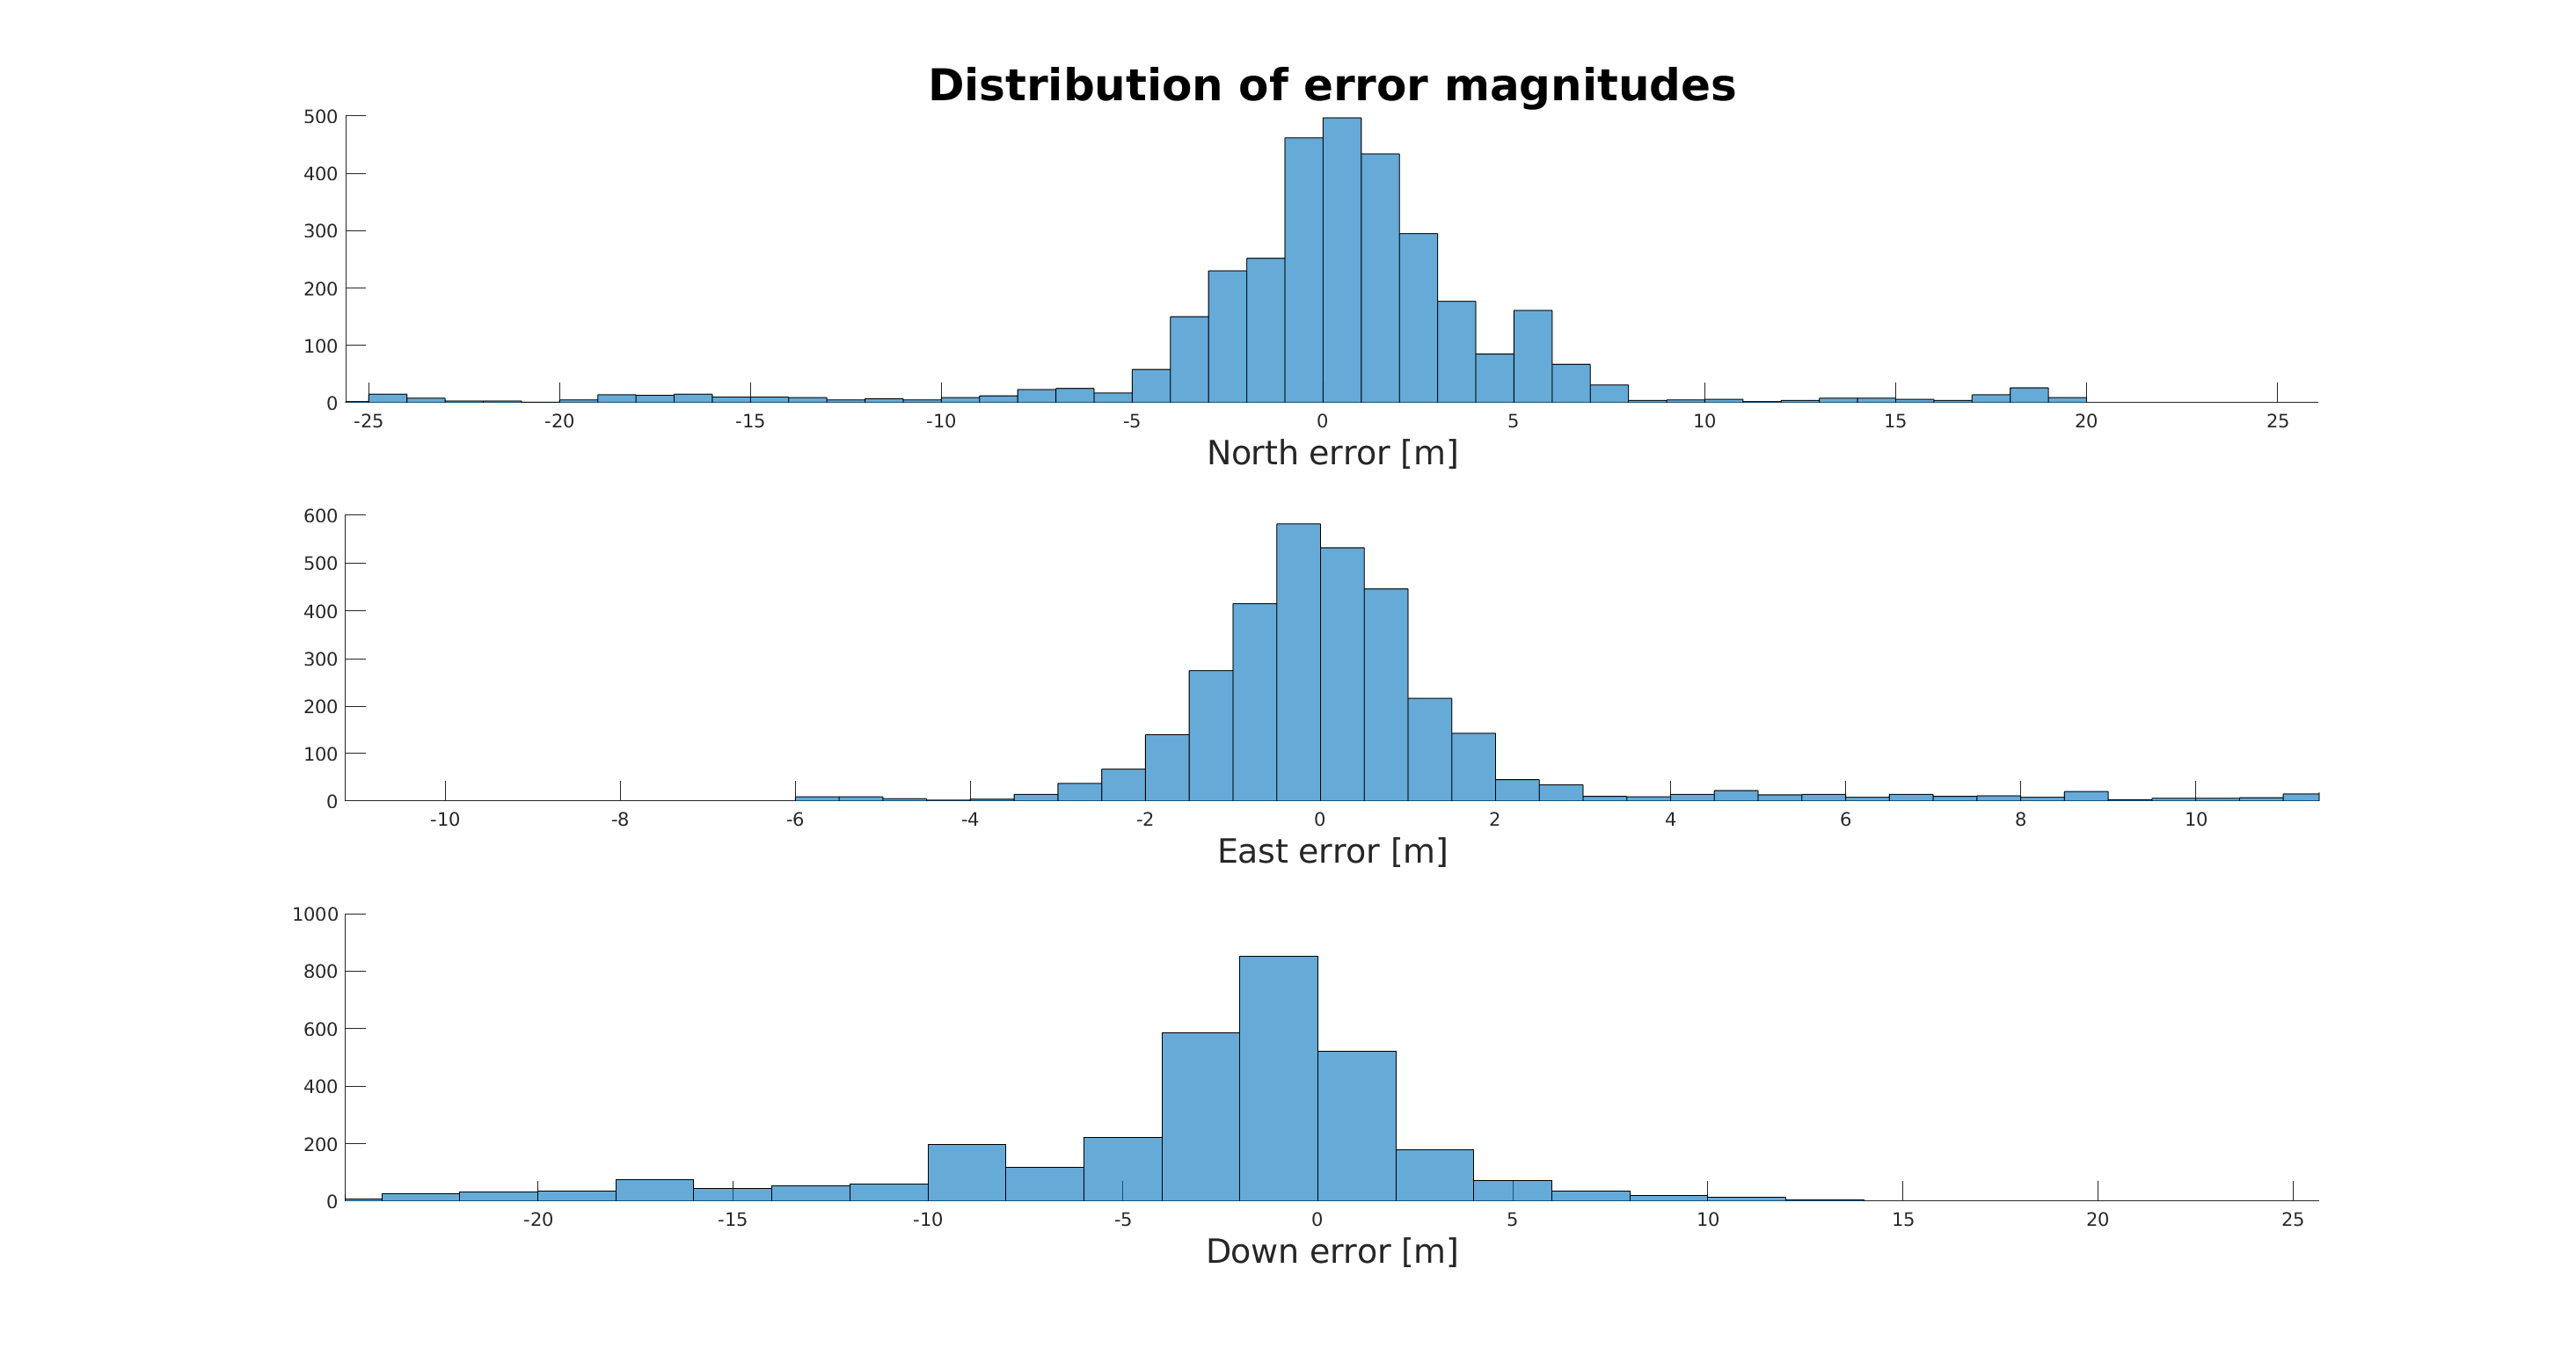
\includegraphics[scale=0.3]{Results/Images/error-hist.eps}
        \caption{Histogram showing the distribution of the position error during testing.}
        \label{fig:error-hist}
    \end{figure}
    
    \begin{figure}[!htbp]
        \hspace{-1.5cm}
        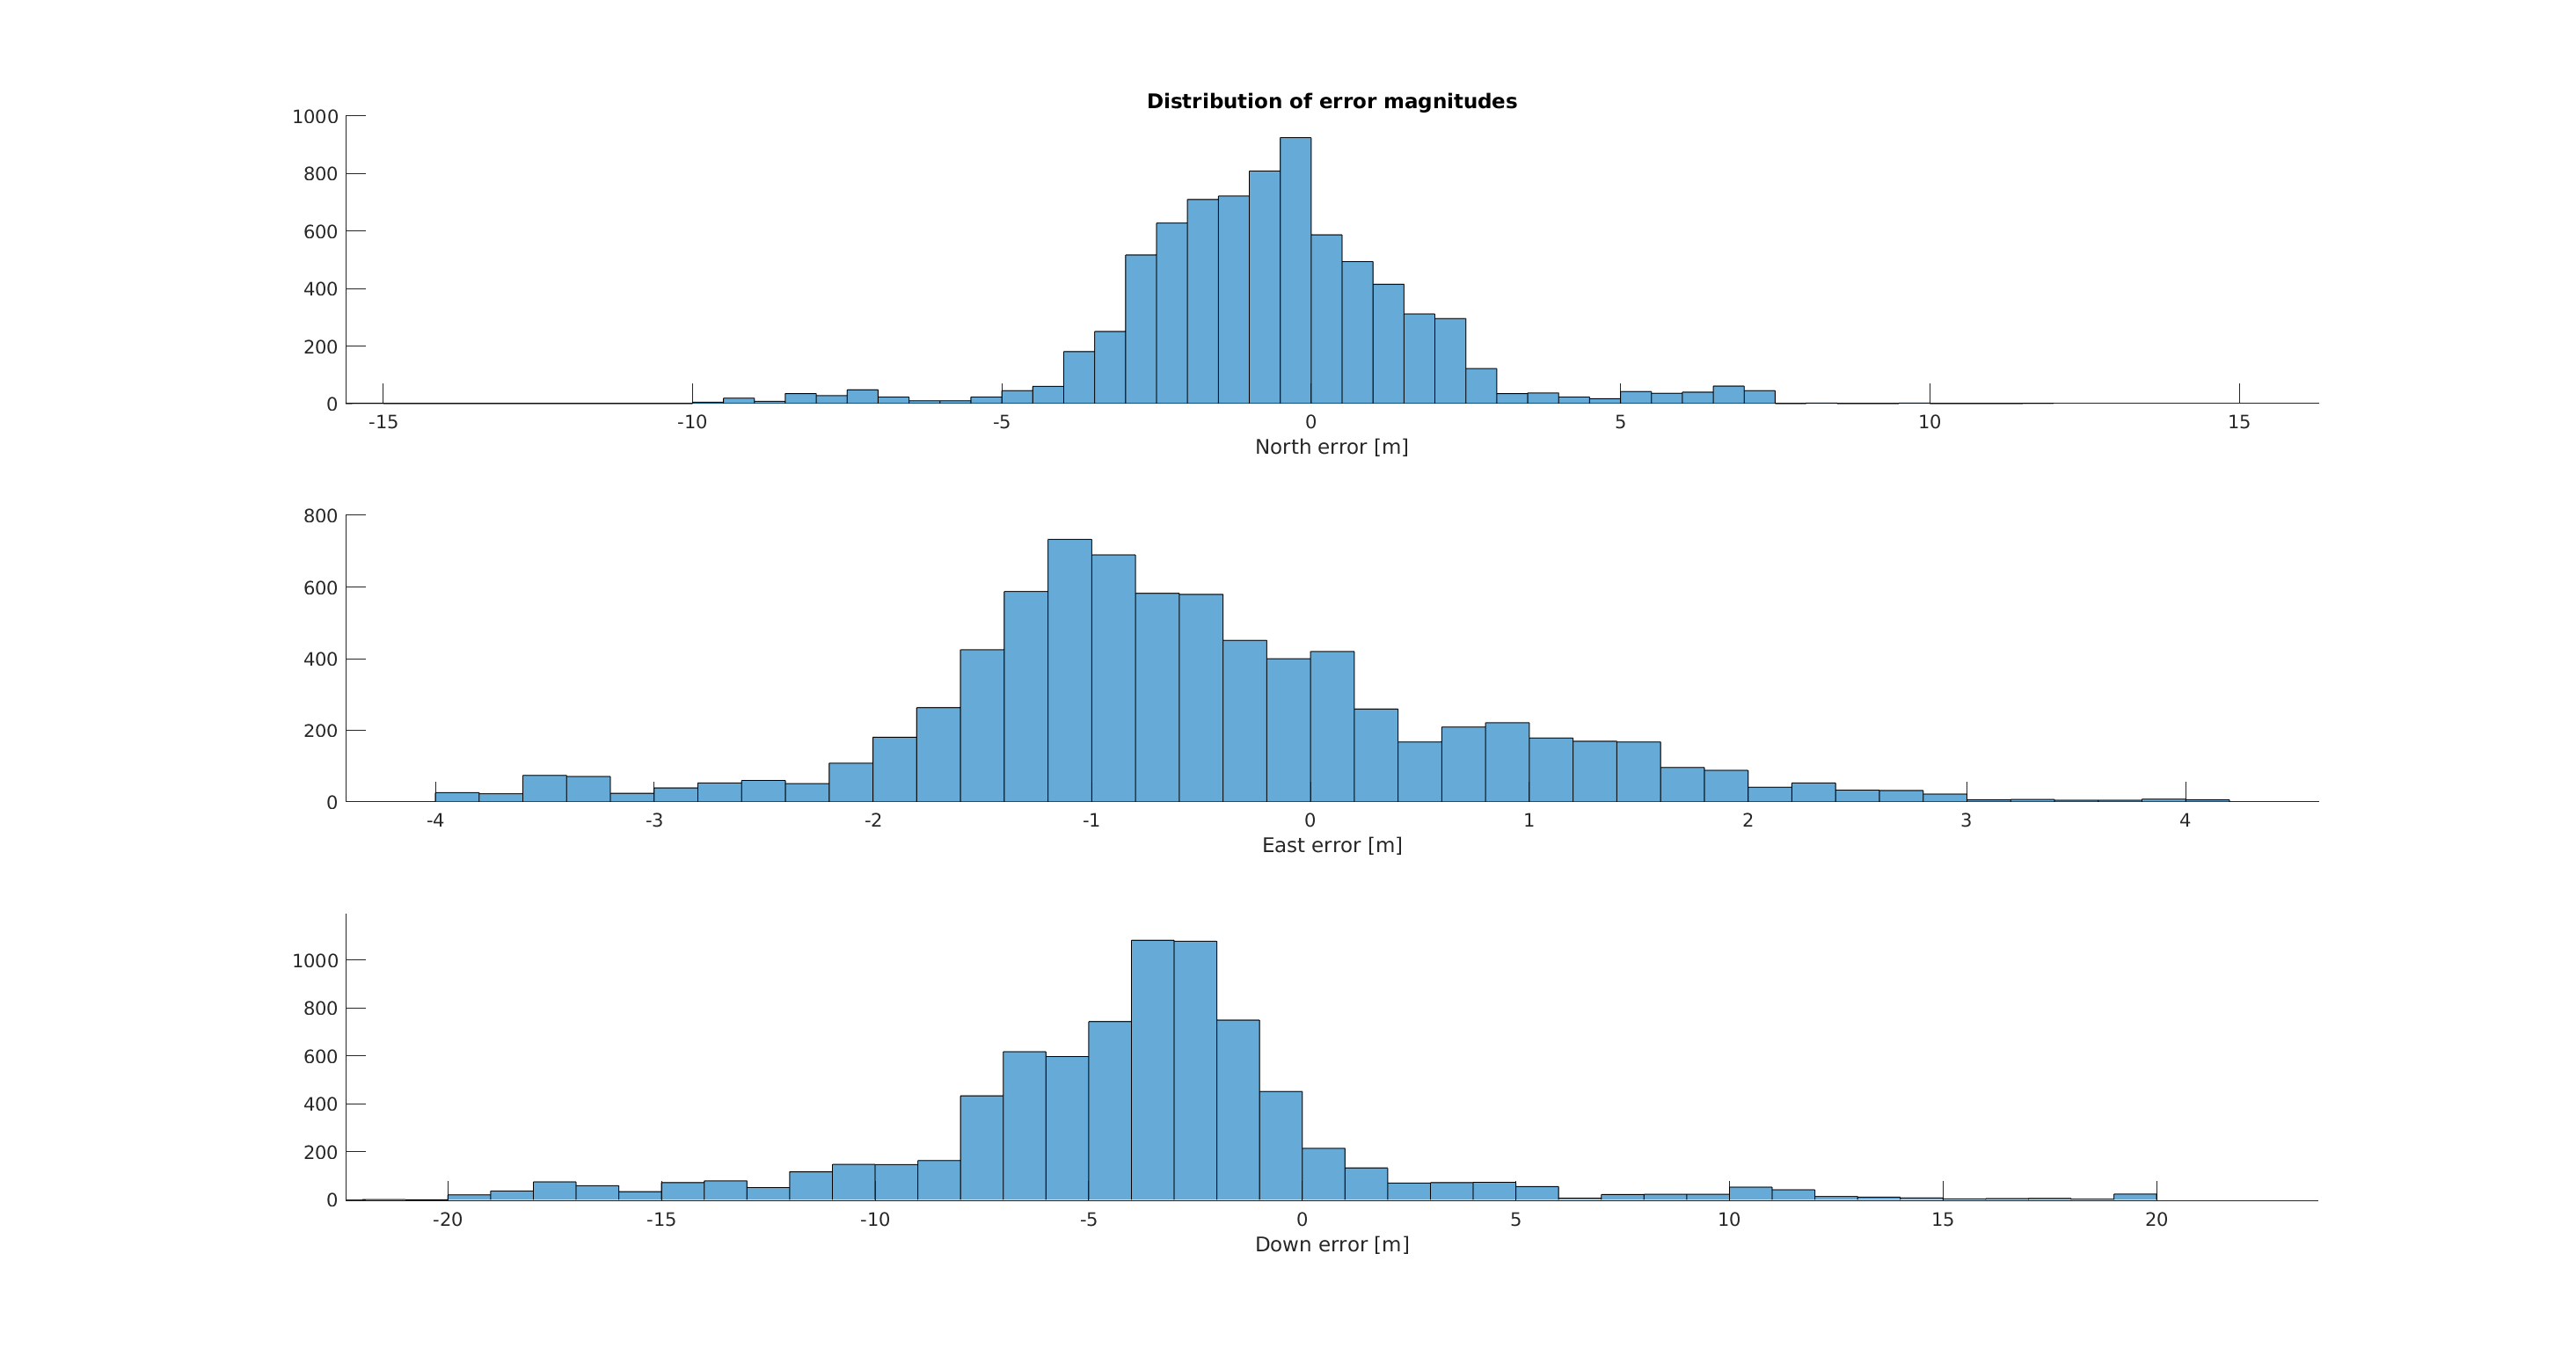
\includegraphics[scale=0.3]{Results/Images/error-hist-gnss.eps}
        \caption{Histogram showing the distribution of the position error of the estimate based solely on GNSS measurements.}
        \label{fig:error-hist-gnss}
    \end{figure}
    
    \begin{figure}[!htbp]
        \hspace{-1.5cm}
        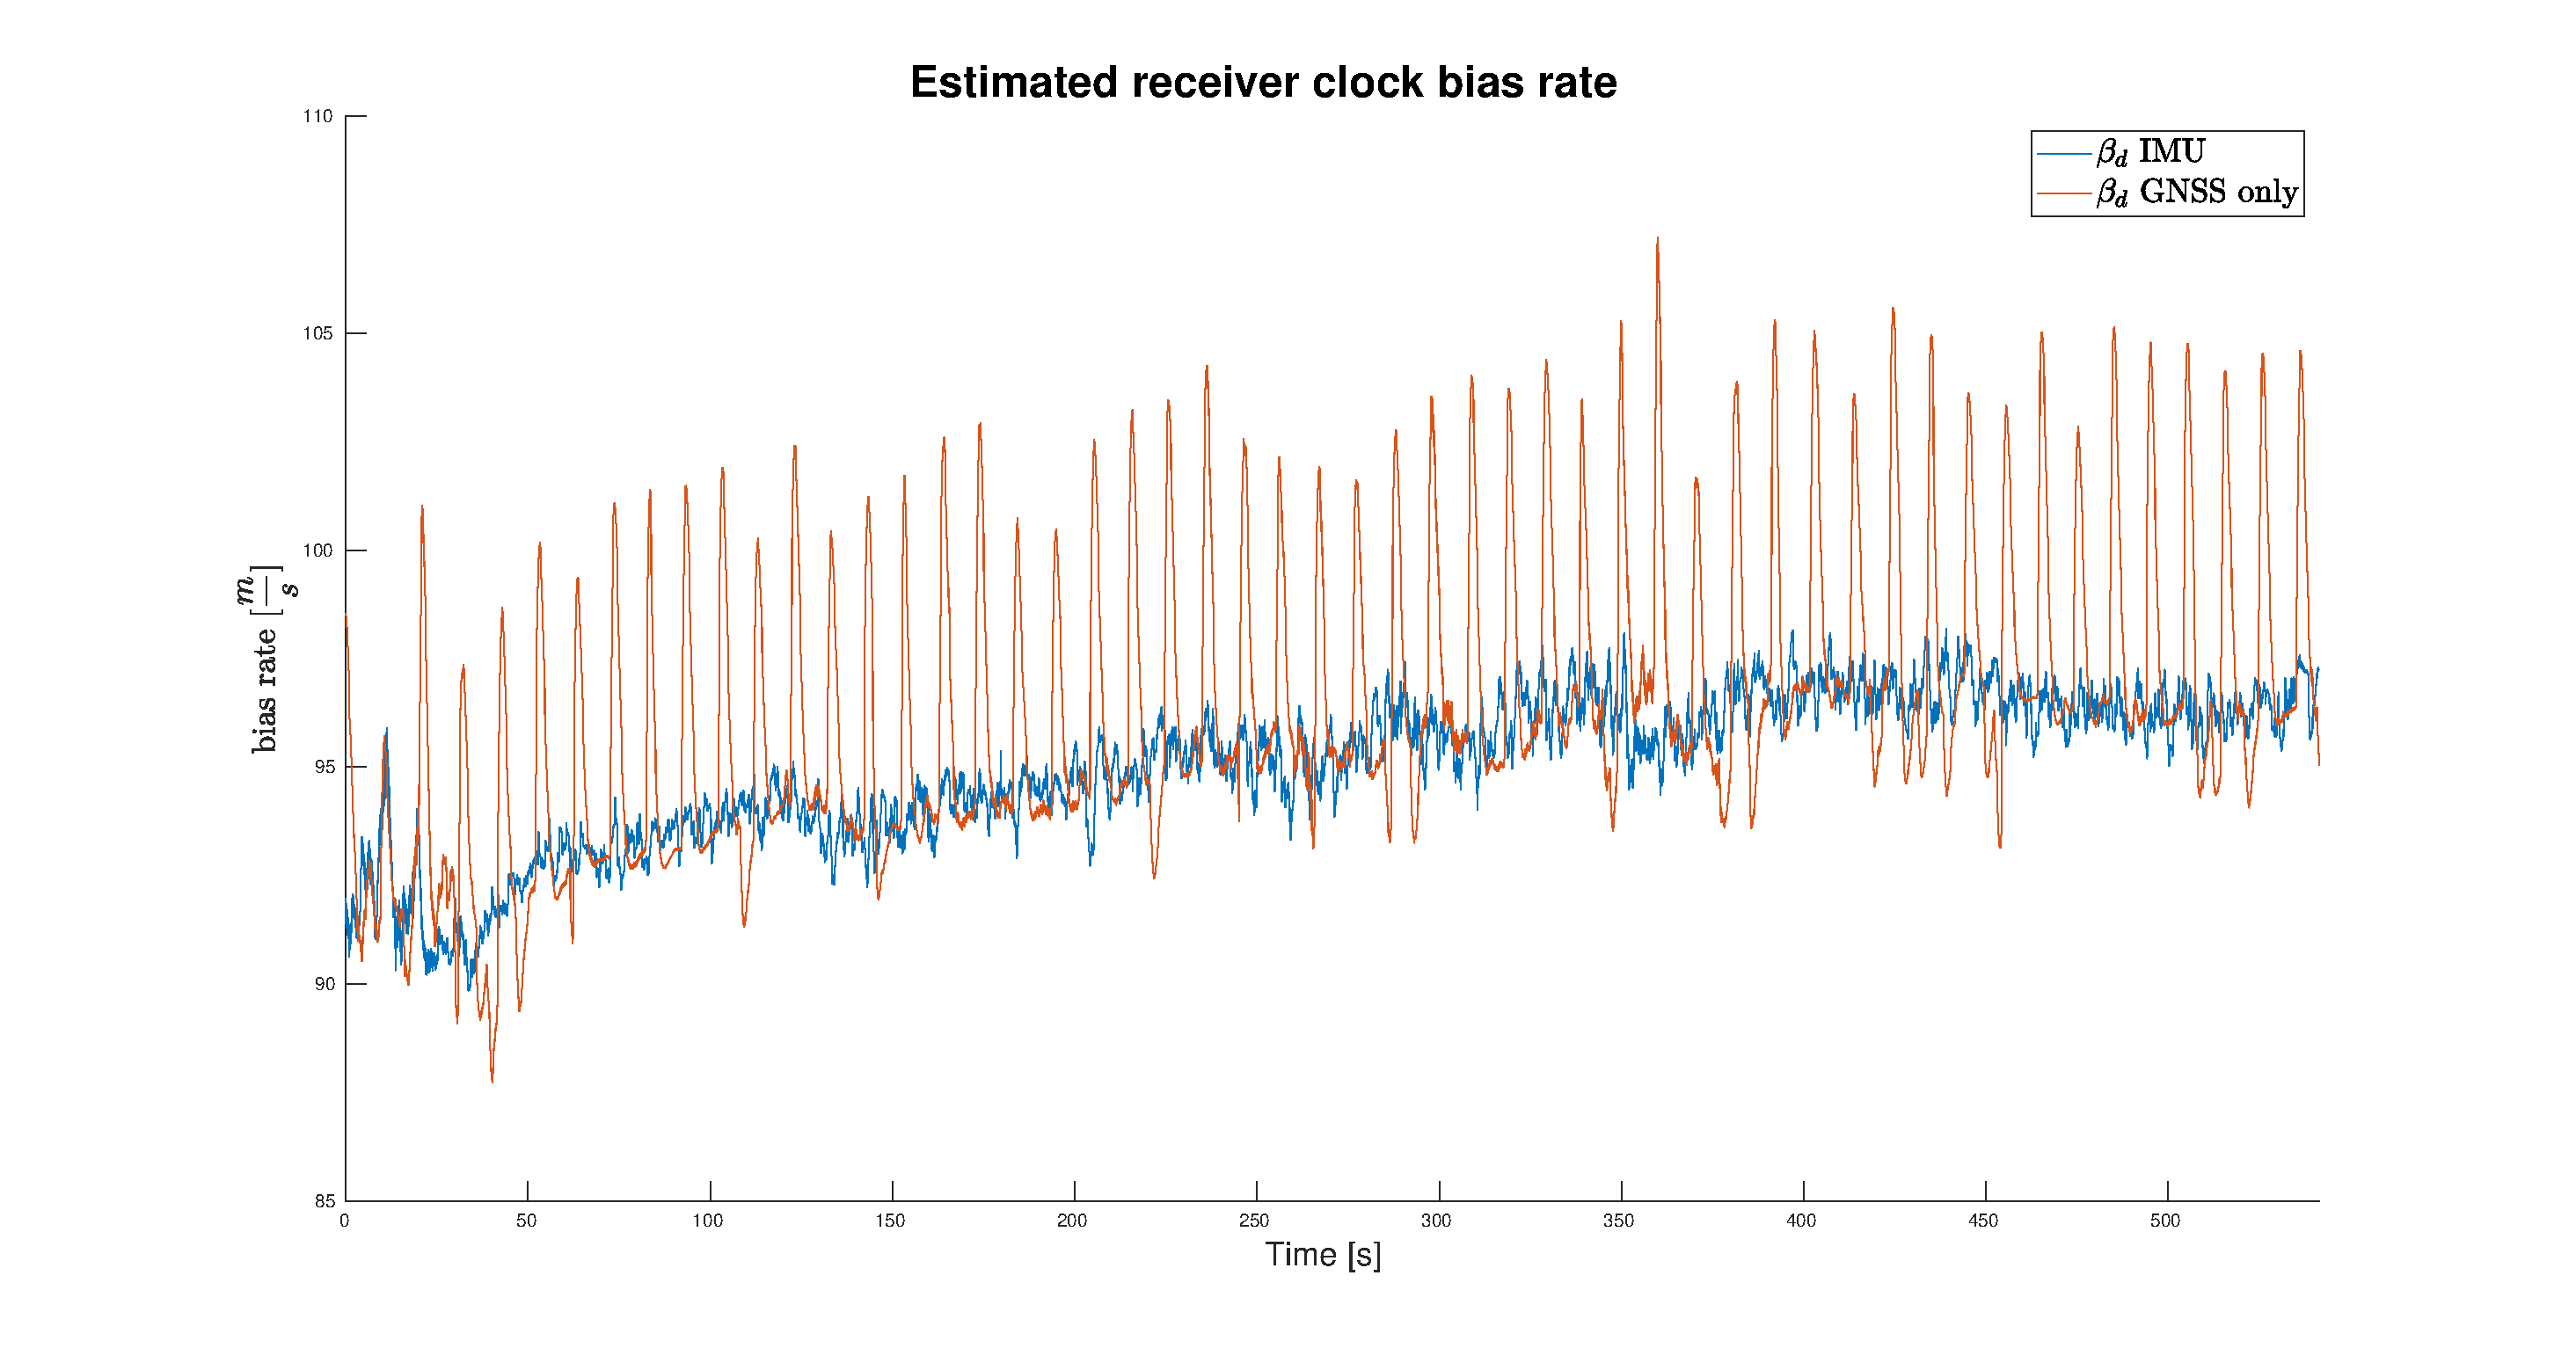
\includegraphics[scale=0.3]{Results/Images/bias_rate.eps}
        \caption{Estimated receiver clock bias rate with and without acceleration measurements.}
        \label{fig:bias-rate}
    \end{figure}
    
    %The errors of the EKF and PixHawk position estimates with respect to the RTK solution are shown in figure \ref{fig:pos-err-sub}. 
    
    \subsection{Multi-GNSS}
    \label{sec:res:multi-gnss}
    It is interesting to note the increase in the amount of available satellites from adding GLONASS measurements. This is shown in figure \ref{fig:n-sat}. Note that this is the number of tracked satellites after the elevation mask is applied. In this case, the number of available satellites are more than doubled, and the tracking of the GLONASS satellites is more stable.\\
    
    \begin{figure}[!htbp]
        \hspace{-1.5cm}
        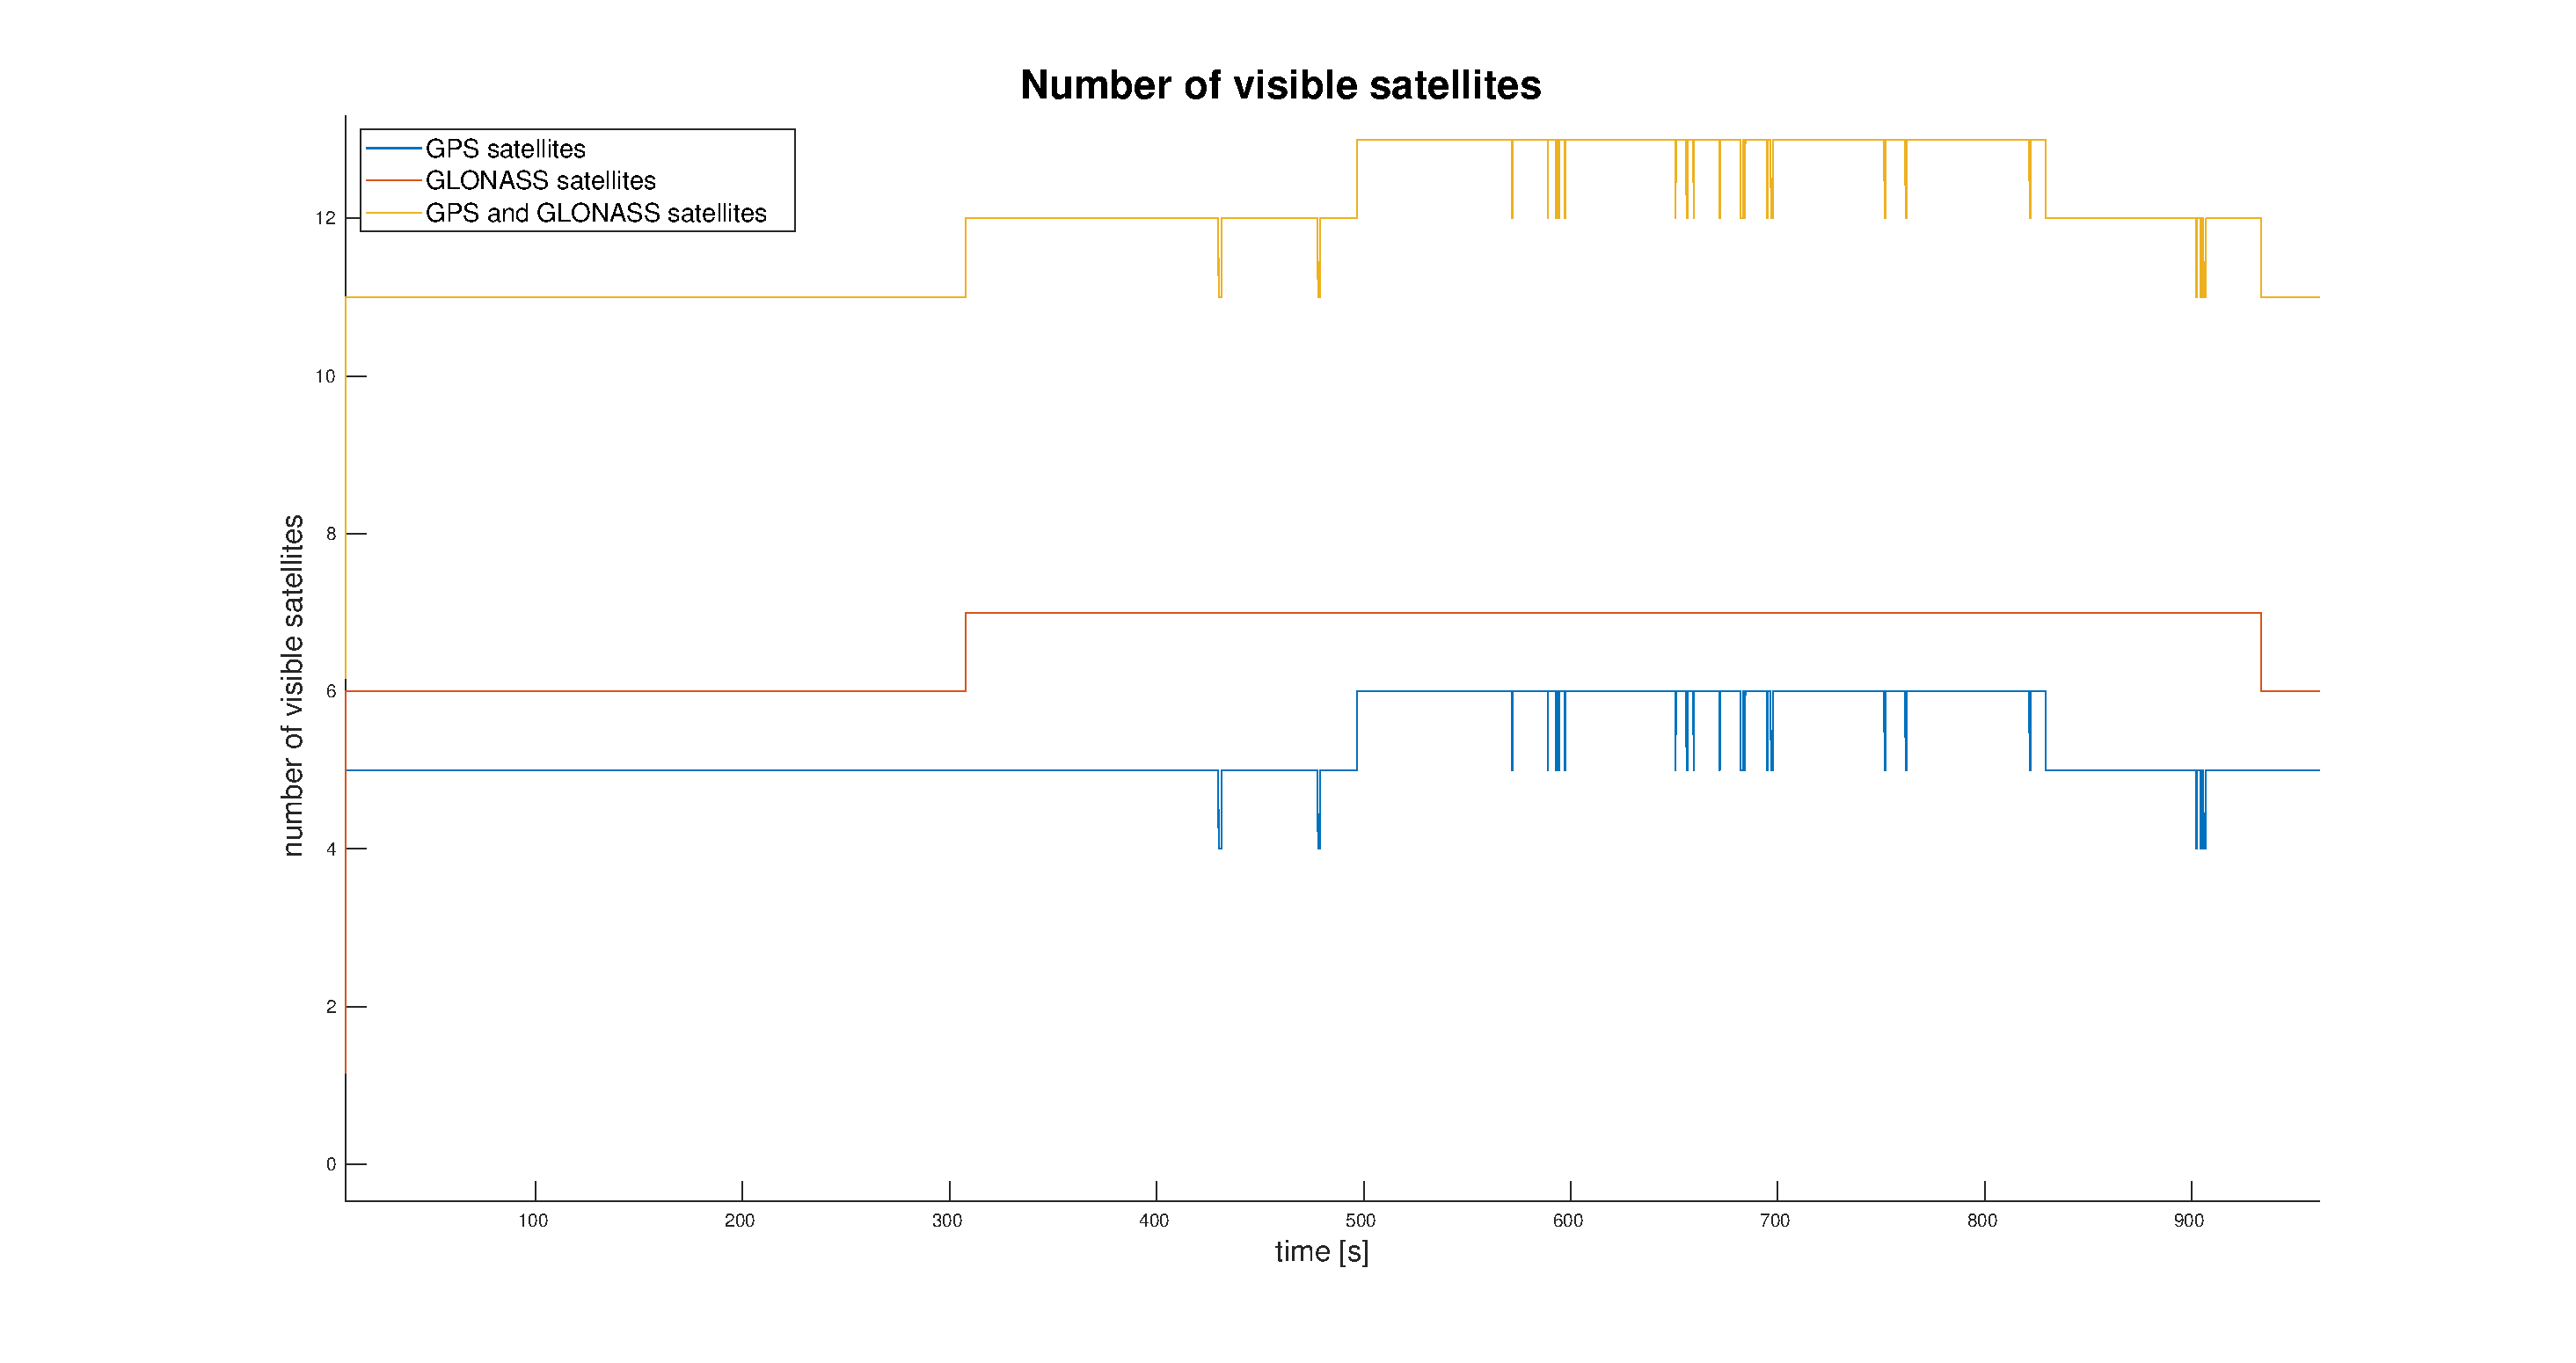
\includegraphics[scale=0.3]{Results/Images/n-visible.eps}
        \caption{Number of tracked GLONASS and GPS satellites during testing}
        \label{fig:n-sat}
    \end{figure}
    
    To investigate the benefits of multi-GNSS, three different setups were tested for the EKF using GNSS only. Nameley, GPS and GLONASS at 10 Hz, only GPS at 10 Hz and lastly, both GPS and GLONASS at 5 Hz. The RMSE values of the position errors are shown in table \ref{tab:rmse-gnss}. Configuring the GNSS receiver to employ both GPS and GLONASS seems to result in a slightly lower RMSE. The postion errors, with respect to the RTK reference, are shown in figure \ref{fig:pos-err-gnss}. Figure \ref{fig:gnss-vel-map} shows the estimated latitude and longitude of the solution obtained from employing both GPS and GLONASS measurements at 10 Hz.
    
    \begin{table}[!htbp]
        \centering
        \begin{tabular}{|c|c|c|c|}
            \hline
            \textbf{Setup} & \textbf{North} & \textbf{East} & \textbf{Down}\\
            \hline
            GPS and GLONASS 10 Hz &  2.3733  &  1.3300  &  6.4983\\
            GPS 10 Hz & 3.4710 &   1.5723 &   6.8607\\
            GPS and GLONASS 5 Hz & 2.5865  &  1.3967 & 6.9490\\
            \hline
        \end{tabular}
        \caption{RMSE values with different GNSS receiver configurations.}
        \label{tab:rmse-gnss}
    \end{table}
    
    \begin{figure}
        \hspace{-1.5cm}
        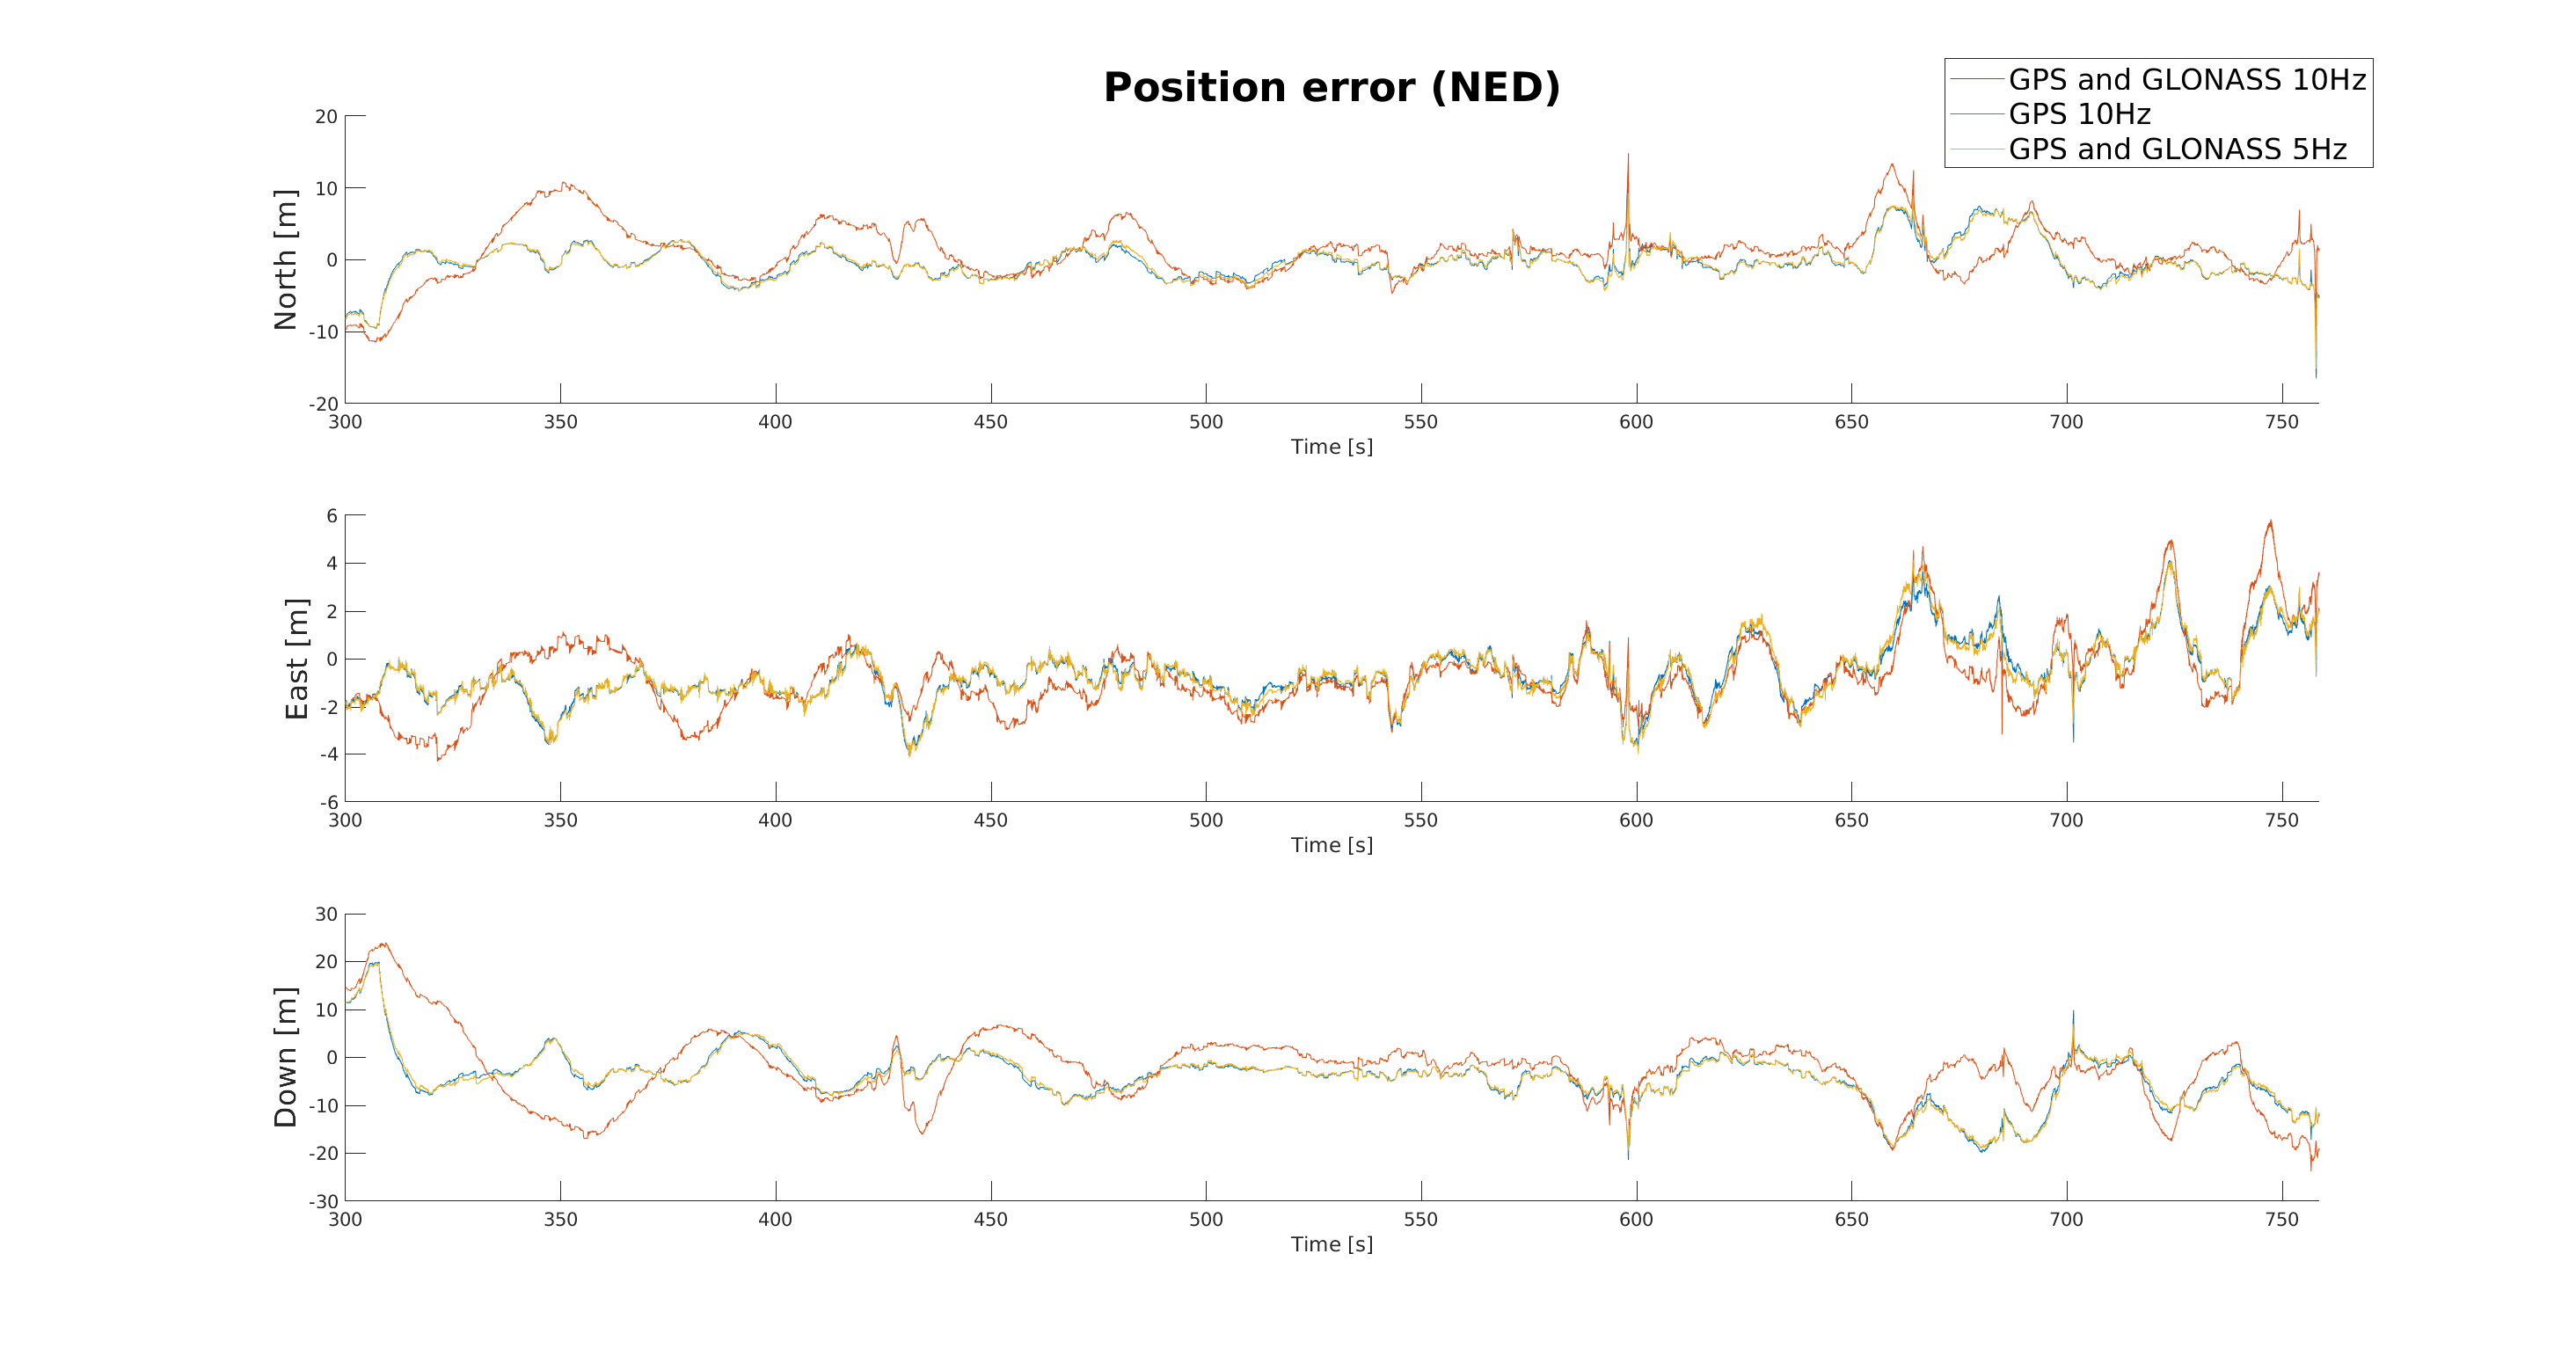
\includegraphics[scale=0.3]{Results/Images/position-err-gnss.eps}
        \caption{Position error of the multi-GNSS setup with different configurations.}
        \label{fig:pos-err-gnss}
    \end{figure}
    
    \begin{figure}[!htbp]
        %\centering
        \hspace{-1.5cm}
        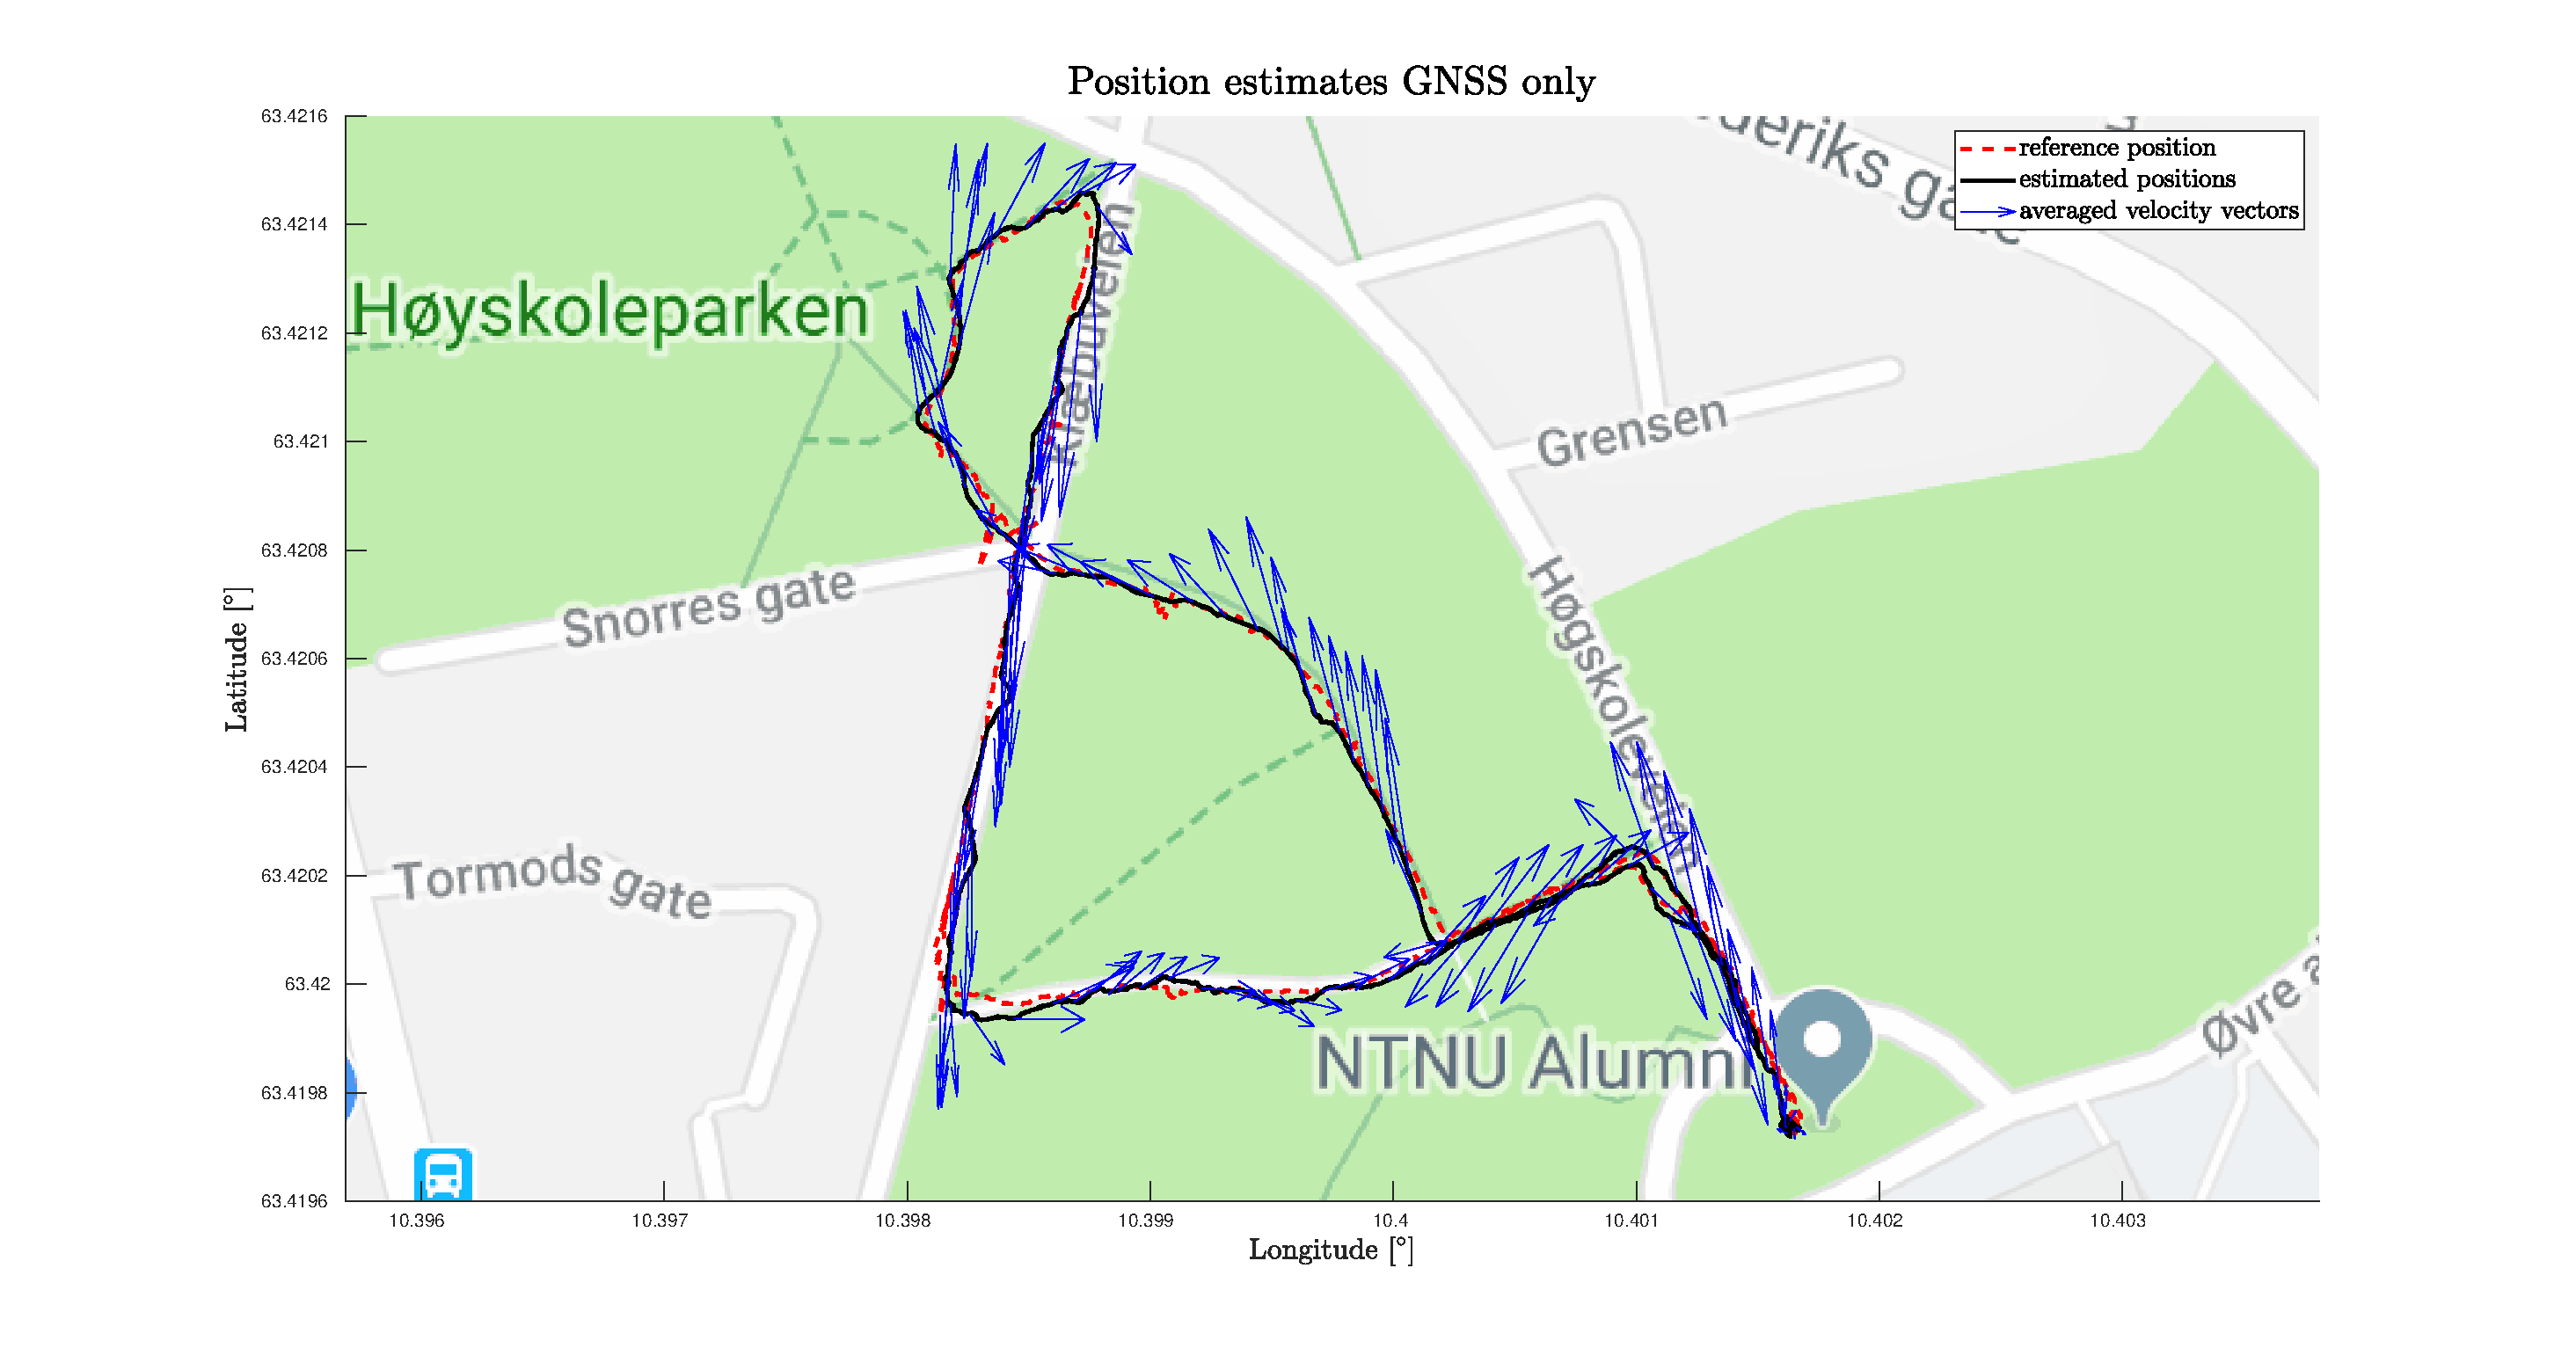
\includegraphics[scale=0.3]{Results/Images/gnss-only-with-vel.eps}
        \caption{Position estimates with averaged velocity vectors from the solution based only on GNSS measurements.}
        \label{fig:gnss-vel-map}
    \end{figure}
    %IMU and GNSS compared with reference path
    %velocity quiver plots in map
    
    %Position subplots compared with rtklib and px
    
    %number of Available satellites GPS, GPS & Glonass
    
    %cpu usage
    
    
    
    
    
    
    
    
    
    
    
    
    
    
    
    
    
    
    
    
    
    
    
    
    
    
    
    
    
    
    
    
    
    
    
    
    
    
    
%\begin{comment}
%\section{Performing the tests}
%To compare the MEKF with other systems several tests were devised, keeping in mind known %limitations of each of the systems. 
%\todo{Describe tests and thoughts behind them}

%\begin{table}[!htbp]
%\caption{List of tests}
%\label{tab:tests}
%    \begin{tabular}{|l|l||p{5cm}|}
%        \hline
%        \textbf{Tested systems} & \textbf{Test description} & \textbf{Expected result}\\
%        \hline
%        Coupled/uncoupled & Circular pattern & The MEKF should show an increase in %precision compared to the     single GNSS solution.\\
%        \hline
%        Indirect/direct filter &  Highly dynamic zigzag motion & The MEKF should follow %the quickly changing     state better than the direct filter.\\
%        \hline
%        The full system & Straight line motion/square pattern & The MEKF should generally %perform better than     the other systems\\
%        \hline
%    \end{tabular}
%\end{table}%
%
%\todo{Describe test environment}
%\missingfigure[]{Ottobil}

%Structure
    % 1 - Introduction
    %     + Test location
    %     + List of compared systems
    % 2 - Performing the tests
    %     + Description of how the tests were performed (waited for steady state..)
    % 3 - Actual results
    %     + Graphs, tables, rms
    %     + 
    
\todo{Log cpu usage}

%\end{comment}

%This chapter presents the experimental results from running the system described in chapter \ref{ch:implementation}. A base station with a setup similar to the described system was set up, and the results are compared to the RTK solution of RTKLIB, as well as the internal PixHawk state estimate.
\newpage
    
\graphicspath{{Appendices/}}
\begin{appendices}
\chapter{Reference frames}
    \subimport{Appendices/}{reference-frames.tex}

\chapter{Hardware}
    \subimport{Appendices/}{hardware.tex}
    
\chapter{Atmospheric models}
    \subimport{Appendices/}{klobuchar.tex}
\end{appendices}
    
\bibliographystyle{abbrv}
\bibliography{bibliography.bib}
    
\end{document}


%x Introduction
%x  - Frontpage
%x  - Abstract
%x  - Sammendrag
%x  - List of figures/tables
%x  - Nomenclature/abbreviations

%x Theory
%x  - GNSS (raskt renskrevet fra prosjektoppgave)
%x  - Integration
%x     1 - Motivation
%x         + Improving state estimation
%x     2 - Architectures
%x         + Loose
%x         + Tight
%x         + Ultra tight
%x         + Feedback vs open loop
%x     3 - Kalman filter
%x         + KF / EKF
%x           - Indirect implementation
%x               - Orientations state minimal. No over-parametrization
%x               - Operating close to the origin. Far away from singularities
%x               - Always small. Second-order products negligible
%x               - Error dynamics are small. All large dynamics already in nominal state. Can apply
%x               - corrections at a lower rate than predictions 
%x               - \cite{sola2017quaternion}
%x           - MEKF
%x               - Maintains quaternion unit length
%x         + Nonlinear observer(?)
%x     4 - Parametrizations
%x         + Vector-angle
%x         + Euler
%x         + Quaternion (Linear diff. eq. No EKF divergence)
%x         + Gibbs
%x         + Modified Rodrigues
%x         + Cayley parameters?
    
% Implementation
%x  - Toolchain
%x     1 - Dune, Neptus, IMC
%x     2 - Glued
%x     3 - RTKLIB
%x  - Hardware
%x     1 - Beaglebone black
%x     2 - Shield 3.0
%x     3 - GNSS receiver
%x  - Simulators
%x     1 - GNSS simulator
%x     2 - Flightgear
%x         + Changing of ardupilot code
%x  - Full system
%x     1 - EKF method description
%x         + Because the expected error state is always zero except between a measurement correction and              the injection of the error in to the nominal state, followed by a reset, there is no poin                in actually implementing the propagation of the error state. The covariance of the error is              however propagated (Ingen x priori)
%x     2 - Paremetrization description and state vector forms
%x         + Quaternions have 3 DOF, but four parameters. P might be rank deficient                                   \cite{trawny2005indirect, sola2017}
%x         + Gibbs vector has a singularity at 180\deg. 
%x     3 - Model description (matrices and functions)
%x         + Discretization \cite{van1978computing, wahlstrom2014discretizing}:
%x     4 - Observability
%x     5 - Noise models
%x         + Eksponentielt synkende støymodell (V1*e^-T1*t + V2*e^-T2*t + V3)
%x     6 - Challenges
%x         + Discretization timestep

%x Results
%x     1 - Introduction
%x         + Test location
%x         + List of compared systems
%x     2 - Performing the tests
%x         + Description of how the tests were performed (waited for steady state..)
%x     3 - Actual results
%x         + Graphs, tables, rms

%x Discussion
%x     1 - Introduction
%x         + Testing goals
%x Conclusion